\documentclass[preprint,nocopyrightspace]{sigplanconf-noauthor}
\usepackage[T1]{fontenc}
\usepackage{graphicx}
\usepackage{xspace,url}
\usepackage{algorithmic}
\usepackage{algorithm}
\usepackage{multirow,color}
\usepackage{subfigure}
\usepackage{amsmath}
\usepackage{amsfonts}
\usepackage{alltt}
\usepackage{amsmath}
\usepackage{comment}
\usepackage{listings}
\lstset{
  language=C++,
  basicstyle=\scriptsize\ttfamily,
  % emph={foreach},
  % emphstyle=\textbf,
  morekeywords={size\_t, token\_t},
  numbers=left,
  showstringspaces=false,
  escapechar={@},
  keywordstyle=\color{blue},
  %stringstyle=\color{magenta},
  commentstyle=\color{red},
  morecomment=[s][\color{red}]{[[}{]]}
}
\usepackage{tabularx}

%\usepackage[sort&compress]{natbib}

%\newcommand{\subparagraph}{}
\usepackage[compact]{titlesec}

\newtheorem{theorem}{\noindent {Theorem}}{}
\newtheorem{lemma}{\noindent {Lemma}}{}
\newtheorem{claim}{\noindent {Claim}}{}
\newtheorem{observation}{\noindent {Observation}}{}
\newtheorem{definition}{\noindent {Definition}}
\newtheorem{problem}{\noindent {Problem}}{}
\definecolor{gray}{rgb}{0.5,0.5,0.5}
\definecolor{MyBlue}{rgb}{0.1,0.3,0.75}
\newcommand{\note}[1]{\textcolor{red}{\bf \em #1}}
%\newcommand{\comment}[1]{{\color{gray}[\textsf{#1}]}}
\newcommand{\authorcomment}[1]{\iffalse #1 \fi}
\newcommand{\etc}{\emph{etc.}\xspace}
\newcommand{\ie}{\emph{i.e.,}\xspace}
\newcommand{\eg}{\emph{e.g.,}\xspace}
\newcommand{\etal}{\emph{et al.}\xspace}
\newcommand{\bfem}{\bf \em}

\newcommand{\vrisha}{{\sc Vrisha}\xspace}
\newcommand{\wukong}{{\sc WuKong}\xspace}
\newcommand{\lancet}{{\sc Lancet}\xspace}

\DeclareMathOperator*{\argmin}{arg\,min}

\newcommand\vartextvisiblespace[1][.5em]{%
  \makebox[#1]{%
    \kern.07em
    \vrule height.3ex
    \hrulefill
    \vrule height.3ex
    \kern.07em
  }% <-- don't forget this one!
}

%caption for table
%\newcommand{\mtcaption}[1]{\caption{#1}\vspace{-0.1in}}
%\newcommand{\mfcaption}[1]{\vspace{-0.03in}\caption{#1}\vspace{-0.25in}}
%\newenvironment{mytable}{\begin{table}}{\vspace{-0.15in}\end{table}}
%\newenvironment{mytable*}{\begin{table*}}{\vspace{-0.15in}\end{table*}}

% TODO: it would be nice to not have to do this
%\linespread{0.972}

\begin{document}

\authorpermission

%\titlebanner{banner above paper title}        % These are ignored unless
%\preprintfooter{short description of paper}   % 'preprint' option specified.

\title{Efficient Load Test Generation}

\authorinfo{Bowen Zhou \and Milind Kulkarni \and Saurabh Bagchi}
           {Purdue University}
           {\{bzhou, milind, sbagchi\}@purdue.edu}

\maketitle

\pagenumbering{arabic}
\pagestyle{plain}

\begin{abstract}

A crucial part of any software testing regimen is {\em performance testing}:
a program must be put under load, \eg by executing a critical loop of the program many times, to
ensure that the program behaves as expected at large scales. Unfortunately,
generating precise performance tests, where a specific part of the program can be 
exercised at a controllable load level, is challenging. The standard approach to generating
performance tests using dynamic symbolic execution incurs too much overhead to
effectively generate large-scale test inputs. We propose \lancet, a dynamic
symbolic execution--based tool that sidesteps the overheads. \lancet has two
key innovations: (i) a path exploration heuristic for dynamic symbolic
execution that more effectively generates scaling inputs for loops in complex
programs; and (ii) a novel {\em constraint inference} method, that uses
statistical inference on small-scale inputs to automatically infer constraints
that describe large-scale inputs, allowing programmers to generate
large inputs without performing symbolic execution at large scales. We
demonstrate the effectiveness of \lancet by using it to infer large-scale,
targeted inputs for synthetic benchmarks and real-world distributed applications
such as Memached and Redis.

\end{abstract}

% \category{D.2.4}{Software Engineering}{Software/Program Verification}[Statistical Methods]
% \category{D.2.5}{Software Engineering}{Testing and Debugging}[Diagnostics]
%  
% \terms
% 
% \keywords

\sloppy

\section{Introduction}
%XXX write about a single idea in a paragraph, only assemble the paragraphs later

%it is difficult to write scalable software?
Writing correct and performant software running at scale has always been a challenge, especially so given the rising popularity of multithreaded and distributed systems.
Scalability turns out to be the Achilles heel of many, otherwise well-designed software systems, which suffer from correctness or performance problems when executed at a large scale.
For example, Foursquare, a geo-social network for sharing experiences of places, had an unprecedented 17 hours of downtime because the data stored in one of its two MongoDB shards reached the hosting computer's RAM capacity~\cite{foursquare-outage}.
This is an example of a scaling problem with the data size.
As another example, the Hadoop Distributed File System (HDFS) runs into performance problems when the number of clients becomes too large, relative to the processing power of the namespace server~\cite{hdfs-scalability}.
This is an example of a scaling problem that is triggered by a large number of nodes, and indirectly, by large sizes of data.
% TODO
% Play low on the importance of input size for two reasons: (a) it is unknown if the satisfiability problem of string constraints with length operations is decidable in general~\cite{z3str-fse13}; (b) there is no off-the-shelf solver that supports string length.

%where high-coverage unit tests fail?
Bugs often happen out of the frequent paths of a program, rather in places where less attention has been paid to in the development process.
As a remedy, unit tests are often introduced to cover both hot and cold paths and check for errors in the runtime.
An important quality criterion for a unit test suite is code coverage, or how much portion of the entire code base of the system under test (SUT) is touched by a test suite.
By the conventional definition of code coverage, a line of code is considered covered if it is executed for at least once by a test.
Such definition of code coverage is fraudulent in two means.
First, it is purely a control flow concept and therefore completely ignorant to the data flow.
For example, a null pointer dereference error may never be triggered by a unit test that exercises the line of code but with a valid pointer.
Furthermore, running every part of SUT for once is not sufficient to reveal many performance issues.
For example, there was a scalability issue in a LRU cache implementation of MySQL~\cite{mysql-49177}, which can only be detected by running SQL SELECT in a loop for a large number of times.


%why performance tests are difficult to write?
Performance testing, as one kind of system testing that performs end-to-end black-box testing, is designed to find performance issues in software.
The idea in its essence is to run SUT through a large input, measure the sustainable performance and observe if any failure is triggered in the runtime.
For simple programs, it is obvious that a larger input will invoke a longer execution.
For example a string copy takes more time for a longer input string.
However, it requires years of practice before one can master the black art of finding "large" inputs for complex real-world software systems.
Sheer increasing the amount of data contained in the input does not necessarily lead to a longer execution, depending on how the program processes the input data.
Take the classic binary search algorithm for example, its run time grows as a logarithmic function of the input size.
To double the run time of binary search, the input must be an order of magnitude larger in size.
On the other hand, more data means more logs, which are more difficult to analyze if a bug does occur.
Numerous research projects invested in log analysis~\cite{oliner-cacm12} have proved the task a difficult one.


%QA's pain
It is only natural to ponder if it is possible to achieve a long execution or a load spike with a reasonably sized input for SUT, or how to push an execution to the limit with inputs of a certain size.
Unfortunately, there exists no systematic method to the best of our knowledge that leads to a performance test that induces a significant level of workload on SUT, not to mention striking a balance between execution length and input size.
QA engineers often need to understand the internals and interfaces of complex software systems that consist of a pile of distributed components and millions of lines of code written by other developers, then endure a lengthy trial-and-error session to find a performance test of good quality.
If we take a closer look, the QA workflow consists of the following steps:
(a) making the test plan, i.e. starting with simple tests focused on individual code paths, followed by combination of different paths to simulate real user behaviors;
(b) understanding the relevant code path and every other part of SUT that interacts with it to get sufficient knowledge for creating the performance tests;
(c) developing and running the performance tests, while measuring the resultant performance using profiling tools.
Out of these steps, (a) defines the policy, or the goal for the performance tests, for which human effort is indispensable, while (b) and (c) provide the mechanisms that implement and verify the resultant performance tests, which also form the most laborious part of the process for QA engineers.

%lancet's contributions which should be echoed in evaluation
We introduce \lancet, a performance test generation tool, to address the pain in the search process of performance tests by automating the latter two steps in the QA workflow where computers can be more efficient than human beings.
\lancet is built on top of symbolic execution and statistical prediction, providing a tool with:
(a) low entry barriers, i.e. little knowledge of SUT internals is required to create good performance tests,
(b) systematic algorithms to reason the performance impact of values in the input,
(c) integrated statistical models to extrapolate the scaling trend of SUT,
(d) support for widely used concurrent and event-driven programming libraries,
(e) on-the-fly SUT instrumentation for measurement and verification of generated performance tests.
By default, \lancet inspects every loop in a program and tries to find inputs to run each loop for the number of iterations specified by the user.
In the case where the user is familiar with the implementation of SUT, he can designate a set of target loops or even a single loop to reduce the scope of code considered by \lancet and speed up the test generation process.
The reason for choosing loops is twofold. %TODO need more work
First, programs spend a large part of their execution time in loops.
Second, we observe, through examination of applications that have had documented scalability problems~\cite{XXX}, as the application is run at larger scales, the negative impact of inefficient or incorrect code inside a loop often gets amplified into severe performance regressions or cascading failures.

When applying \lancet to an application, the user can specify the loop he wants to test and the load level, \ie the number of iterations, for the loop.
\lancet takes these parameters from the user as guidance to steer its symbolic execution engine and finds the inputs that reach the given number of iterations for the given loop.
\lancet makes two changes to the state-of-the-art symbolic execution algorithm.
First, to reach a specific number of iterations after entering the target loop, \lancet uses a loop-centric search heuristic that favors the paths that stay inside the loop over those that exit.
This path prioritization strategy is in contrast to existing path strategies that favor finding new paths.
Second, \lancet shortcuts the path exploration by applying statistical inference to derive the path constraints at a large number of iteration from training samples, which consist of path constraints from running the loop a small number of iterations.
This way, to reach $N$ iterations of a given loop, \lancet just needs to execute the loop for 1 $\ldots$ $M$ iterations where $M \ll N$ and collect the constraints at each iteration. Afterwards, the constraint solver is invoked for the extrapolated path constraints to get the input that would trigger $N$ iterations of the target loop.

%TODO update the apps
We apply \lancet to four disparate programs: a linear algebra code, {\tt mvm}, a quantum computer simulator from SPEC, {\tt libquantum}, a fluid dynamics program, {\tt lbm}, and a utility from the GNU Coreutils suite, {\tt wc}.
Each of these programs needs to scale up to satisfy common use cases: {\tt mvm} to tackle large matrices, {\tt lq} to factorize large numbers, {\tt lbm} to simulate flows for more timesteps, and {\tt wc} to process large text corpuses.
We show that for these programs, \lancet is able to generate more, and larger-scaling, inputs than a state-of-the-art test generation tool when given the same amount of computation time, and that in all cases, \lancet can generate even larger inputs through the use of statistical inference.
Moreover, because of the regularity of the constraints that \lancet performs inference over, it is able to make its predictions perfectly, allowing programmers to correctly generate inputs of any size without incurring the cost of additional symbolic execution.

\paragraph{Outline}
Section~\ref{sec:background} provides background on symbolic execution.
Section~\ref{sec:method} describes the basic design of \lancet, using a simple matrix-vector multiplication program as an example.
%Section~\ref{sec:extensions} discusses how we extend \lancet to support more general programs, including those with many symbolic inputs and those that operate over structured input, while
%Section~\ref{sec:discussion} explains the remaining shortcomings of \lancet.
Section~\ref{sec:implementation} sketches the implementation of \lancet.
Section~\ref{sec:evaluation} presents case studies of using \lancet to generate large-scale performance tests for several real-world applications.
Section~\ref{sec:related} discusses related work, and
Section~\ref{sec:conclusion} concludes.







%%% old intro starts here
%%% TODO move symbolic execution material into overview


% Many programs suffer from scalability problems
%Many software systems are called on to scale to large sizes, both in terms of sizes of data and numbers of application processes that are part of the system. Scalability also turns out to be the Achilles heel of many, otherwise well-designed software, whereby they suffer from correctness or performance problems when executed at a large scale. There are myriads of examples of this reported in bug repositories~\cite{hadoop-6901, cassandra-4681}, and in a few cases, they have caused widespread end-user visible outages. For example, Foursquare, the site for sharing experiences of places using geo-tagged information, had an unprecedented 17 hours of downtime because the data that it stored in MongoDB NoSQL store went through a spike causing problems with its sharding solution \cite{foursquare-outage}. This is an example of a scaling problem with the data size. As another example, the Hadoop Distributed File System (HDFS) runs into performance problems when the number of servers over which the data is spread becomes too large, relative to the number of servers used to store the meta-data \cite{hdfs-scalability-problem}. This is an example of a scaling problem that is triggered by a large number of nodes, and indirectly, by large sizes of data. 

% \begin{comment}
% Scalability is a key requirement for programs that aim to process ever-increasing amount of data and span thousands of nodes, especially in the wake of the diminishing increase in single-core performance and the broad adoption of multicore and scale-out architectures. Whether a program is scalable in terms of the size of input or the number of processors depends on a variety of possibly intertwined factors such as hardware specification, program behavior and workload characteristics. As a result of this complexity, minor mistakes in implementation and overlook of system peculiarities can dramatically hinder a program from running correctly and efficiently at scale. Thus, it is desirable to conduct systematic scalability testing of the program before releasing it into production.
% \end{comment}

% How to stress test programs for scalability
%So the question arises what is the best way to stress test an application to uncover the scalability problems during testing? Today, there exists a wide variety of robust tools for stress testing applications, through variants of workload generators \cite{box-test, faban, httperf, jmeter, rubis, olio}. Through these, the developer\footnote{We use the term ``developer'' with the understanding that the activity may be carried out by a ``developer'' rather than the original developer. We will not make a distinction between these two roles for this paper.} can introduce a certain controlled amount of load as input to the application and observe the effect on the application. For example, given a certain rate of users that perform write transactions, what is the throughput of the application. As another example of stress testing that is widely used today, given a certain artificially introduced constraint on the resource available to an application (such as, reduced memory), what is the effect on the application performance~\cite{nagaraja-usits03}. However, consider the use case that the developer would like to target a specific region of code, such as, a computationally demanding loop, and would like to stress test the application by running the loop a user-driven (large) number of times. {\em Existing software testing approaches are not able to support this use case.}

% SB (11/10/13): CTM - check white box testing literature
% Why the use case of LANCET is important
%The above use case comes up in many situations --- where the developer suspects a loop to be causing the slowdown as she tests the program at various scales, or where the developer would like to investigate the behavior of some specific, seldom-exercised code region, such as, exception handling code. In these use cases, the developer would like to ``direct'' the stress test generation framework to the specific region of code, and then to perform the test in a specific manner, such as, by causing a loop to iterate a given number of times. In this paper, we seek to provide such functionality in an efficient manner. We then wish to use this functionality to generate stress tests for evaluating scalability of real, complex programs. 

% \begin{comment}
% In practice, programmers conduct stress testing with the help of workload generators~\cite{box-test, faban, httperf, jmeter, rubis, olio} to measure the performance of an application and find QoS violations or functional bugs at high loads. During a testing session, a programmer wants to measure the performance of the application at given levels of loads (also called load testing), or find functional or performance anomalies under extreme conditions such as workload spike, resource starvation, or hardware failure. She imposes no control over which part of the application to be tested but rather treats the program as a black box. To increase the chance of finding functional or performance issues triggered by extreme demand, the programmer tweaks the workload generator in an ad-hoc manner to create long-running test cases that bombard the application with a large amount of data.

% The black-box approach is agnostic to the internal logic of the application under test other than the input and output interfaces. Without the knowledge of how data is processed at different points of the program, stress testing essentially takes the {\em nuke-it-from-orbit} method by pumping into the program as much data as possible, burning lots of CPU cycles in repetitive invocations of the hot paths, to see if anything breaks. However, the frequent paths is also the part of code which is developed with extra care and tested extensively, hence less likely to have problems. Even for the case where a bug is successfully discovered using the black-box approach, it would save a lot of time and effort if we could uncover the same bug in a much shorter testing session with a carefully crafted input that press the vulnerable code with just enough load.
% \end{comment}

% Tie-in to symbolic execution
%The field of symbolic execution \cite{exe-ccs06,dart-pldi05,klee} provides us with a basic building block for providing the functionality described above. Symbolic execution \cite{sen-cacm} is typically used in software testing to explore as many different program paths as possible in a given amount of time, and for each path to generate a set of concrete input values exercising it. Then, at specific points in each path, it can insert checks for the presence of various kinds of errors including assertion violations, uncaught exceptions, security vulnerabilities, and memory corruption. The key idea behind symbolic execution is to use {\em symbolic values}, instead of concrete data values, as input values, and to represent the values of program variables as symbolic expressions over the symbolic values. As a result, the output values computed by a program are expressed as a function of the input symbolic values. Relevant to our desired goal, symbolic execution can explore different program paths and through a constraint solver that it employs, it can generate the actual (\ie concrete) input values needed to exercise a given path. 

% \begin{comment}
% Recent development in symbolic execution~\cite{exe-ccs06,dart-pldi05} enables white-box test generation tools like KLEE~\cite{klee} to produce high-coverage tests for popular applications such as GNU/Coreutils. These tools represent the input to a program as an array of symbolic variables, accumulating constraints on the symbolic variables at each conditional branch that depends on the input, solving the set of constraints at the end of each execution path to get a concrete input that would trigger the same path if given to the program. Symbolic execution tools resort to SMT solvers~\cite{stp, z3} to determine which branch to pursue at every conditional branch or if it is necessary to fork a new path if both branches are satisfiable for the current set of constraints, which makes it intractable for them to explore long paths that contain a lot of branches due to the {\em path explosion} problem. Previous researches~\cite{cloud9,burnim-icse09,zhang-ase11} proposed methods to speed up the process by parallelizing symbolic execution of different paths or pruning uninteresting branches based on heuristics. However, they still need to execute the whole path symbolically, which makes them unsuitable for the search of long-running execution paths.
% \end{comment}

% Why symbolic execution cannot satisfy our requirement 
% However, the latest developments in symbolic execution still fail to meet our requirements for generating stress tests for scalability evaluation. This arises from the fact that what we would like to do is to be able to execute a {\em given} loop a {\em given} number of times. We {\em do not} care to explore all paths needed to reach this loop and we {\em do} care to execute the loop a given number of times, which is typically a large number since we are testing for scalability. Symbolic execution is focused on path coverage and biases its search through a program's code path to identify hitherto unseen paths. This is without doubt an important aspect of software testing, but it does not support the use cases for scalability testing that we have laid out above. Further, symbolic execution runs into the problem of path explosion, since the number of program paths grows (roughly) exponentially with program length%
% % \footnote{Actually, number of conditional branch points in a program, to 
% % be precise.}
% . Thus, if we were to tweak symbolic execution to iterate a loop a given number of times, it will generate constraints for symbolic variables for {\em each} loop iteration. Thus, the number of constraints will quickly grow to a large number and solving them will become prohibitively expensive. Keep in mind that solving constraints to generate the concrete values from the symbolic variables is the most computationally expensive part of symbolic execution. 

% Our solution - why we target loops
% In this paper, we present \lancet, which incorporates the developer's insight to generate stress tests targeted at performance-critical code in complex real-world applications. We build \lancet using the basic principle of symbolic execution, as described above, but modify it fundamentally to remove its shortcomings with respect to our goal of stress testing for scalability. Specifically, \lancet generates stress tests for loops. The reason for choosing loops is twofold. First, programs spend a large part of their execution time in loops.
% % , as has also been reported for a wide variety of domains \cite{lhotak-popl11,feng-pldi12}. 
% Second, we observe, through examination of applications that have had documented scalability problems, that often there are critical loops that are executed more frequently as the application is run at larger scales. The negative impact of inefficient or incorrect code inside a loop often only manifests when the loop is executed a specific, typically large number of times.

% can only be brought out by causing the loop to execute a controlled, typically large, number of times. 

% \begin{comment}
% First, loop is the smallest syntax unit of a program that gets executed for more times when larger inputs are given to the program, which means the program would spend more time running inside loops as it scales up. As a result, the efficiency of code insides loops is critical to the scalability of the whole program. On the other hand, most programs spend a big chunk of their execution time inside loops, as pointed out by previous research~\cite{lhotak-popl11}. For example, a web service usually enters an infinite loop waiting for incoming requests after the initial setup steps is finished. A cluster scheduler would go through a queue of tasks and schedule each of them to the most suitable node, which all happens in a task scheduling loop. The negative impact of inefficient or incorrect code inside a loop can only be amplified by the repetition.
% \end{comment}

% Use case of our system; contributions to speed up execution
% When applying \lancet to an application, the programmer can specify the loop she wants to test and the load level, \ie the number of iterations, for the loop. \lancet takes these parameters from the programmer as guidance to steer its symbolic execution engine and finds the inputs that reach the given number of iterations for the given loop. The typical use case would be to run the loop a {\em large} number of times. For this, \lancet makes two changes to ordinary symbolic execution. {\em First}, to reach a specific number of iterations after entering the target loop, \lancet uses a loop-centric search heuristic that favors the paths that stay inside the loop over those that exit. This path prioritization strategy is in contrast to existing path strategies that favor finding new paths. {\em Second}, \lancet shortcuts the path exploration by applying statistical inference to derive the path constraints at a large number of iteration from training samples, which consist of path constraints from running the loop a small number of iterations. This way, to reach $N$ iterations of a given loop, \lancet just needs to execute the loop for 1 $\ldots$ $M$ iterations (in a discontinuous manner through the range) where $M \ll N$ and collect the constraints at each iteration.
% To reach the target loop, \lancet employs a classical path searching strategy that mixes random path selection and code coverage heuristics.

% Demonstration
% We implement \lancet by extending KLEE, the most widely used symbolic execution tool. We apply it to four disparate programs: a linear algebra code, {\tt mvm}, a quantum computer simulator, {\tt libquantum}, a fluid dynamics program, {\tt lbm}, and a Unix text utility, {\tt wc}. Each of these programs needs to scale up to satisfy common use cases: {\tt mvm} to tackle large matrices, {\tt lq} to factorize large numbers, {\tt lbm} to simulate flows for more timesteps, and {\tt wc} to process large text corpuses. We show that for many programs, \lancet is able to generate more, and larger-scaling, inputs than KLEE when given the same amount of computation time, and that in all cases, \lancet can generate even larger inputs through the use of inference. Moreover, because of the regularity of the constraints that \lancet performs inference over, it is able to make its predictions perfectly, allowing programmers to correctly generate inputs of any size without incurring the cost of additional symbolic execution.

 % --- a numeric program \texttt{libquantum}, which is a quantum computer simulator; Unix utilities \texttt{grep} and \texttt{wc}; and \texttt{Blast}, the widely used program from NIH for matching genomic sequences. Each of these programs needs to scale up to satisfy common use cases --- \texttt{libquantum} is used to factorize large numbers; \texttt{grep} and \texttt{wc} are used with large text corpuses; and \texttt{Blast} is used for matching in large genomic databases. We show through experimentation that with a cutoff time of XXX hours, KLEE is only able to generate inputs for scales of XXX, XXX, and XXX, while \lancet can generate inputs for scales XXX, XXX, and XXX. A statistical inference procedure always has inaccuracies and we see that our inaccuracy is only XXX for these three applications. Here accuracy refers to the ability to generate valid inputs, \ie, inputs that will indeed let the loop execute the user-given number of times. 
 
% \paragraph{Outline}
% Section~\ref{sec:background} provides background on dynamic symbolic execution. Section~\ref{sec:method} describes the basic design of \lancet, using a simple matrix-vector multiplication program as an example. Section~\ref{sec:extensions} discusses how we extend \lancet to support more general programs, including those with many symbolic inputs and those that operate over structured input, while Section~\ref{sec:discussion} explains the remaining shortcomings of \lancet. Section~\ref{sec:implementation} sketches the implementation of \lancet. Section~\ref{sec:evaluation} presents case studies of using \lancet to generate large-scale performance tests for several real-world applications. Section~\ref{sec:related} discusses related work, and Section~\ref{sec:conclusion} concludes.

\section{Background: Dynamic Symbolic Execution}
\label{sec:background}

Many state-of-the-art white-box test-generation tools rely on {\em dynamic
symbolic execution}~\cite{klee,dart-pldi05,sen-cacm}. This section provides a brief
overview of how these tools work, and discusses some of the shortcomings of
current techniques that \lancet aims to ameliorate.

\subsection{Dynamic Symbolic Execution Basics}

Dynamic symbolic execution couples the traditional strengths of symbolic
analysis---tracking constraints on variables to determine the feasibility of
various program behaviors---with the efficiency of regular concrete execution.
The inputs to a program are treated as symbolic variables.
% SB (11/12/13): This is better said as ``The inputs to a program are 
% treated as symbolic variables.''
As the program
executes, statements that involve symbolic variables are executed
symbolically, adding constraints on symbolic variables. When a
branch statement is reached ({\em e.g.} {\tt if (x < y) goto L}), {\em one} of
the paths is taken, and the appropriate constraint is added to the {\em path condition}, or set of constraints ({\em e.g.}, if the branch above is taken, the constraint $(x <
y)$ would be added to the path condition). As new constraints are added to the
path condition an SMT solver (Satisfiability Modulo Theory) is invoked to ensure that
the path condition is still satisfiable; unsatisfiable constraints imply that
the particular path that execution has taken is infeasible---no program
execution could follow that path. Once a path through the program is found,
the SMT solver is used to produce a {\em concrete} set of values for all
the symbolic variables. These concrete values constitute an input. Note that
unlike traditional symbolic execution, dynamic symbolic analysis can always
fall back to concrete values for variables; if execution encounters a
statement that cannot be analyzed using the underlying SMT solver, calling an external function for example, the
variables involved can be concretized and the statement can be executed
normally. What it gives up is completeness of the code coverage as a result
of the concretization. 

\subsection{Path Exploration Heuristics}

One of the key decisions in dynamic symbolic execution tool is how to choose
the path through a program an execution should explore. In other words, how to
choose directions for the branches encountered in execution. For example, a
tool such as KLEE~\cite{klee} executes multiple paths concurrently, in an attempt to
generate a series of inputs to exercise different paths of the program.
When encountering the branch statement described above, KLEE can fork the
execution to two clones that follow the two branches respectively, choose one
execution clone to explore first and save the other for later. The resultant
paths would include the constraint $(x < y)$ in the clone that follows the true
branch, and $\neg(x < y)$ in the one that follows the false
branch.


There are numerous heuristics that can be used to choose which path
to explore first at each branch in dynamic symbolic execution; the choice of the
correct heuristic depends on the goals of the particular tool being developed.
We abstract away the goal of a dynamic symbolic execution tool by describing
it in terms of a {\em meta-constraint}. A meta-constraint is a higher level
constraint that the path condition describing a particular execution
attempts to satisfy. For example, in the case of generating high-coverage
tests, the meta-constraint for a tool may be to produce a path that exercises
program statements not seen by previously-generated inputs, in which case a
path-exploration heuristic might prioritize flipping branches to generate a
never-before-seen set of constraints. In the case of generating stress tests,
as in \lancet, the meta-constraint would be to generate a path condition
that exercises a particular loop body a certain, user-defined number of times, in which case
the path-exploration heuristic might prioritize taking branches that cause the
loop to execute again, till the user-defined limit is reached 
(Section~\ref{sec:loop-centric}). Note that just
as a path condition may not be tight---there can be many possible
concrete inputs that follow a particular path through the execution---a
meta-constraint need not be tight: multiple path conditions may all
satisfy a given meta-constraint.

\subsection{Dynamic Symbolic Execution Overhead}

The primary drawback of dynamic symbolic execution is its dependence on an
underlying SMT solver to manage the path condition that an execution generates.
At every branch, the SMT solver must be invoked to determine whether a
particular choice for a branch is feasible or infeasible. Though the
constraint solver is also invoked to concretize input variables when
necessary, or to generate the final concrete input for a particular run, the
majority of queries to the solver arise from these feasibility
checks~\cite{sen-cacm}. Though there are many techniques to reduce the expense
of queries to the constraint solver, such as reducing the query size by
removing irrelevant constraints and reusing the results of prior queries
whenever possible~\cite{klee}, the fundamental expense of invoking the
constraint solver at each branch in an execution remains. This overhead can
lead to an order-of-magnitude slowdown in execution~\cite{klee}.

A second overhead of dynamic symbolic execution is the path-explosion problem.
The path exploration heuristics of a particular tool may prioritize certain
choices for branches in an attempt to satisfy the tool's meta-constraint.
However, the exploration heuristics may be wrong: whenever a branch is
encountered, if the heuristic makes the wrong choice, the meta-constraint may
not be satisfiable, and the tool must return to the branch to make a different
choice.

These two overheads make generating large-scale, long-running inputs using
dynamic symbolic execution difficult. First, as the path being explored gets
longer, more branches are encountered, resulting in more invocations to the
SMT solver. Second, long-running inputs execute more branches, creating more
opportunities for the path-exploration heuristic to ``guess wrong,'' leading
to unsatisfiable meta-constraints and ultimately leading to path explosion.

\subsection{WISE}

WISE is perhaps the most closely-related dynamic symbolic execution technique
to \lancet. WISE attempts to generate worst-case inputs for programs ({\em
e.g.}, a worst-case input for a binary-search-tree construction program would
be a sorted list of integers, generating an unbalanced tree)~\cite{burnim-icse09}. In
meta-constraint terms, WISE attempts to generate a path condition
that produces worst-case inputs of a reasonably large size.

While it is possible to exhaustively search through all possible path conditions for a certain input size to find the worst-case inputs, it is clear that this approach will lead
to path explosion when applied to larger inputs. To avoid the path explosion
problem, WISE uses the following strategy. It exhaustively searches the
input space for small input sizes to find worst-case behaviors. Then, by
performing pattern matching on the worst-case path conditions generated
for different input sizes, WISE learns what choices worst-case path conditions typically make for branches in the program ({\em e.g.}, always following the
left child to add a new element in a BST). This pattern is then integrated
into a path-exploration heuristic.

At large scales, when WISE encounters a branch, it looks through the
patterns that it identified at small scales to choose the direction for the
branch. In essence, WISE has a notion of what a worst-case path condition
``looks like,'' and chooses directions for branches to make the path condition
for a larger input match that worst-case pattern. By using this new
path-exploration heuristic, WISE is able to find worst-case inputs for larger
scales without exploring every possible path. In many cases, WISE need only
explore a single path through the program to find a worst-case input!

WISE addresses the overheads of dynamic symbolic execution by tackling the
second drawback described above: it controls path explosion by learning the
pattern of path constraints from smaller runs where path explosion is less of
an issue. Nevertheless, WISE still sits on top of dynamic symbolic execution,
and must query the SMT solver at every branch; it does not tackle the first
source of overhead. As a result, even though WISE has much better scalability
than na\"ive symbolic execution, it still cannot generate particularly large
inputs. Generating an input that runs a loop one million times still requires
performing symbolic execution on a run that visits the loop test condition one
million times.


Section~\ref{sec:inference-mode} explains how \lancet tackles this
problem. In particular, \lancet can generate large-scale inputs for a program
{\em without ever performing symbolic execution at large scales}.

% \section{Overview of \lancet}\label{sec:overview}



\begin{figure}[tb]
\centering
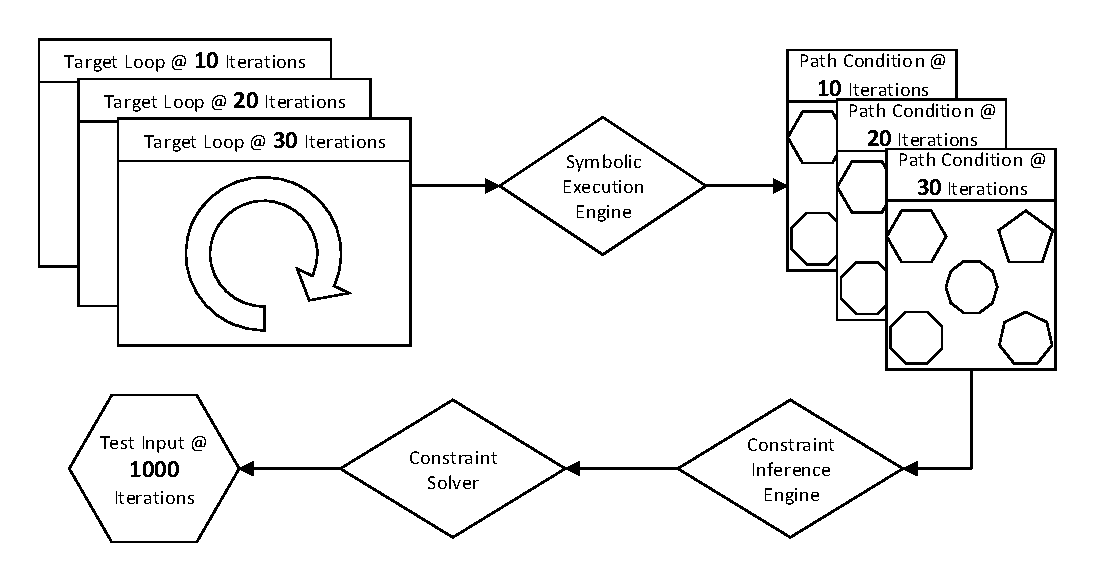
\includegraphics[width=\linewidth]{figures/method}
\caption{High level flow of \lancet's approach for generating inputs to run a loop 1000 times.}
\label{fig:method}
\end{figure}

Figure~\ref{fig:overview} shows the basic operation of \lancet. After the target loop in the program is identified (Section~\ref{sec:target-loop}), \lancet generates a set of path constraints that satisfy a {\em loop-iteration meta-constraint} that the target loop executes exactly $k$ times. For small $k$, this is done by augmenting KLEE~\cite{klee} with a custom {\em loop-centric} path-exploration heuristic (Section~\ref{sec:loop-centric}). 

While traditional dynamic symbolic execution techniques suffice to generate path constraints that run a loop a small number of times, they are impractical for large $k$: running a loop thousands of times will require orders of magnitude more invocations to \lancet's constraint solver than running a loop tens of times, and will be unacceptably slow. \lancet's novel approach to this problem is to determine the path constraints that satisfy the loop-iteration meta-constraint for a large $k$ {\em without performing symbolic execution}.

To achieve this goal, \lancet takes the following steps. First, \lancet generates a {\em series} of path constraint sets, each for different small values of $k$. It then analyzes those path constraints to separate the constraints in those sets into {\em validity constraints}---constraints that ensure that inputs are well-formed---and {\em scaling constraints}---constraints that determine how many times the target loop runs (Section~\ref{sec:validity-constraints}). \lancet then uses the scaling constraints to train a statistical model that relates the value of $k$ to the associated scaling constraints, and uses this model to {\em infer what the scaling constraints would look like} for large $k$ (Section~\ref{sec:constraint-inference}). These inferred scaling constraints are then perturbed slightly to account for modeling error and combined with the validity constraints to produce a new constraint set, which can be solved with a constraint solver, generating a large-scale input for the program (Section~\ref{sec:input-generation}). Crucially, once the initial training phase of \lancet is complete, inputs that target {\em any scale} can be generated at the same overhead (though potentially different levels of accuracy), making \lancet a truly scalable approach to generating large-scale, stress-test inputs.

% The search for a path of a given number of iterations of the target loop begins with executing the program with an arbitrary input, e.g. an existing hand-crafted test case, trying to discover as many new paths as possible with a search strategy that is a mix of random walk and code coverage heuristics, until any of the paths it explored enters the target loop. From there on, \lancet switches to a loop-centric search strategy which prioritizes the paths that keep iterating the loop over those that exit. The path searching process continues until \lancet finds a path that has reached the requested trip count.

\section{Design}\label{sec:method}

\lancet is a dynamic symbolic execution tool that aims to generate {\em scaling inputs} for programs: inputs that cause programs to run for a long time. In contrast to black-box stress-generation tests, \lancet targets particular loops for scaling. It attempts to generate inputs that will cause a chosen loop to execute a specified (large) number of iterations. In this way, particular regions of code can be targeted to see how they behave under heavy load. This section first describes \lancet's behavior at a high level, and then explains \lancet's various components in more detail. %For ease of exposition, this section assumes that there is just one symbolic input parameter in the program under test,\footnote{Note that other variables dependent on this input parameter may also be symbolic} and that parameter is numeric ({\em e.g.}, a single integer parameter). Section~\ref{sec:extensions} discusses how \lancet deals with more general inputs.
For ease of exposition, this section assumes that the program under test takes a single symbolic string as input.
%Section~\ref{sec:extensions} discusses how \lancet deals with more general inputs.

\subsection{Overview of \lancet}
\label{sec:overview}

\lancet has two modes of operation: {\em explicit} mode, which uses traditional dynamic symbolic execution techniques to generate inputs that run a target loop for a specified, small number of iterations, and {\em inference} mode, which uses statistical techniques to generate inputs that run a target loop for a large number of iterations. These modes are described in more detail in Sections~\ref{sec:explicit-mode} and~\ref{sec:inference-mode}, respectively. At a high level, they behave as described next.

\lancet's explicit mode begins by using programmer annotations to identify the target loops (Section~\ref{sec:target-loop}). For each target loop, \lancet then generates a path condition that satisfy a {\em loop-iteration meta-constraint} that the target loop executes exactly $N$ times. For small $N$, this is done by a custom {\em loop-centric} path-exploration heuristic (Section~\ref{sec:loop-centric}).

While the explicit mode suffice to generate path constraints that run a loop a small number of times, it is impractical for large $N$: \eg running a loop a thousand times will require two orders of magnitude more invocations to \lancet's constraint solver than running a loop ten times, and will be unacceptably slow. \lancet's novel approach to this problem is to determine the path constraints that satisfy the loop-iteration meta-constraint for a large $N$ {\em without performing symbolic execution}.

\begin{figure}[tbp]
  \centering
  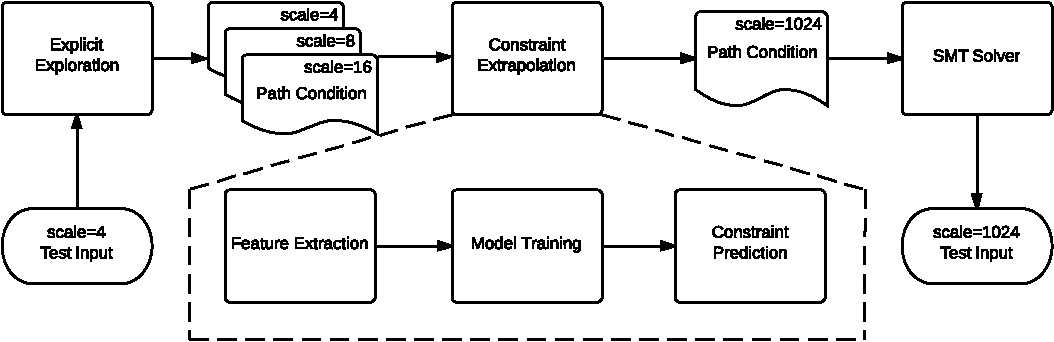
\includegraphics[width=\linewidth]{figures/lancet} %TODO need to update
  \caption{High level flow of \lancet's inference-mode approach for generating inputs for a given loop.}
  \label{fig:method}
\end{figure}

% \lancet's inference mode operates as shown in Figure~\ref{fig:method}. First, \lancet uses its explicit mode to generate {\em multiple} path constraint sets, each for different small values of $N$. It then analyzes those path constraints to separate the constraints in those sets into {\em validity constraints}---constraints that ensure that inputs are well-formed---and {\em scaling constraints}---constraints that determine how many times the target loop runs (Section~\ref{sec:validity-constraints}). \lancet then uses the scaling constraints to train a statistical model that relates the value of $N$ to the associated scaling constraints, and uses this model to {\em predict what the scaling constraints would look like} for large $N$ (Section~\ref{sec:constraint-inference}). These predicted scaling constraints are then perturbed slightly to account for modeling error and combined with the validity constraints to produce a new constraint set, which can be solved with a constraint solver, generating a large-scale input for the program (Section~\ref{sec:input-generation}). 

\lancet's inference mode operates as shown in Figure~\ref{fig:method}.
First, \lancet uses its explicit mode to generate {\em multiple} path conditions, for a pair of consecutive numbers of iterations $M$ and $M+1$, using a symbolic input string of $L$ bytes.\footnote{Multiple path conditions may result in the same number of iterations.}
It then looks into pairs of path conditions for different numbers of iterations and identifies the {\em incremental set}, the set of path constraints that {\em only} exist in the $M+1$-iteration path conditions.
\lancet then extrapolates the path condition of $N$ iterations by appending $N-M$ copies of the incremental set to the $M$-iteration path condition, each projected to appropriate offsets beyond the initial $L$ bytes of the input string using a linear regression model (Section~\ref{sec:constraint-inference}).
Finally, the predicted $N$-iteration path condition is solved with a constraint solver to generate a large-scale input for the program (Section~\ref{sec:input-generation}), which is then verified in real execution of the program. Depending on the result of verification, \lancet may restart the explicit mode to generate more training data and refine the large-scale input based on new path conditions discovered in the explicit mode.

% TODO Move the following to detail sections
% Inference is done on differential constraints produced by the same branch instruction.
% All differential constraints are grouped by the branch instructions that introduce them.
% Though always being introduced by the same instruction, the terms in a constraint may change from iteration to iteration. 
% \lancet applies a separate model to predict the value of each term, concrete or symbolic, for each of the additional $N-M$ iterations.
% If every iteration took the same path through the loop body, the same set of branches, thereby the same path condition would appear again and again.
% Given the number of times each differential constraint appears in a single iteration, \lancet then projects the number of times it would appear should the loop run for $N$ iterations ($N \gg M$).
% Finally, if a different path were taken in an iteration after the first $M$ iterations, the predicted path condition would miss some constraints from the new path, generating inputs that would not be able to reach $N$ iterations or failing to generate any inputs at all because of contradictory constraints.
% In this case, \lancet retreats to the explicit mode to discover more distinct paths through the loop body before going into the inference mode again.

Crucially, once the initial training phase of \lancet is complete, inputs that target {\em any scale} can be generated at the same overhead (though potentially different levels of accuracy), making \lancet a truly scalable approach to generating large-scale, stress-test inputs.

\paragraph{Running example}

% To aid in the discussion of the components and operation of \lancet, we will use a running example of matrix-vector multiply, as shown in Figure~\ref{fig:example}. A few salient points: (i) the code computes $y = A*x$, where $A$ is an $u \times v$ matrix, and $x$ is a $v \times 1$ vector; (ii) though there are two input variables to this code, $u$ is fixed at 10, to satisfy the single-variable constraint mentioned above; (iii) though the size of the matrix and the size of the vector are independent inputs, they are required to be equal to each other, leading to a single degree of freedom in scaling (see Section~\ref{sec:multivar} for more discussion); (iv) though the program generates matrix and vector values, the control flow of the program is independent of those values (see Section~\ref{sec:structured} for how \lancet handles value-dependent control flow).
%
% \begin{figure}[tb]
% \centering
% \begin{lstlisting}
% int u = 10; //input variable, fixed to 10 (* \label{line:u} *)
% int v1 = /* read */; //symbolic, columns in matrix
% int v2 = /* read */; //symbolic, rows in vector

% if (v1 != v2) exit(1); //dimensions match (* \label{line:v1neqv2} *)
% if (v1 <= 0) exit(1); //vector not zero (* \label{line:v1le0} *)

% float A[u][v1] = /* generate random matrix */
% float x[v2] = /* generate random vector */
% float y[v2] = /* initialize vector to zero */

% [[loop_target]] (* \label{line:annotation} *)
% for (int i = 0; i < v1; i++) { (* \label{line:targetloop} *)
  % for (int j = 0; j < u; j++) { (* \label{line:innerloop} *)
    % y[j] += A[j][i] * x[i];
  % }
% }
% \end{lstlisting}
% \vspace{-5pt}
% \caption{Running example: matrix-vector multiply.}
% \label{fig:example}
% \end{figure}

To aid in the discussion of the components and operation of \lancet, we will use a running example of request parsing from Memcached~\cite{memcached}. A few salient points:
(i) the code parses the request string that contains a {\em get} command followed by a list of keys separated by one or more spaces;
(ii) the first function {\tt tokenize\_command} splits the command string (a symbolic string of configurable size received from the Socket layer of \lancet, see Section \ref{sec:socket}) into a list of tokens, stores them as a list of tokens terminated by a length 0 token, then returns the number of tokens retrieved;
%the loop at line~\ref{line:for-loop} scans each byte in the command string, and uses two pointer variables {\tt s} and {\tt e} to pinpoint the start and the end of each token.
(iii) the second function {\tt parse\_get\_command} parses the list of tokens in the target loop (line~\ref{line:while-loop}) and executes the {\em get} command for each key contained in {\tt tokens}.
%Clearly, the number of iterations of the target loop is the same as the number of tokens passed to the function.
(iv) the number of iterations executed by the target loop is determined by the loop in function {\tt tokenize\_command}.
(v) in the following references to this example, we suppose the length of the {\tt command} string is 8 bytes for the ease of exposition.

\begin{figure*}[tbp]
\centering
\begin{lstlisting}
size_t tokenize_command(char *command, token_t *tokens, size_t max_tokens) {
    char *s, *e;
    size_t ntokens = 0;
    size_t len = strlen(command);
    unsigned int i = 0;
    s = e = command;
    for (i = 0; i < len; i++) { @ \label{line:for-loop} @
        if (*e == ' ') { @ \label{line:isspace} @
            if (s != e) { @ \label{line:sneqe} @
                /* add a new token into tokens */
                ntokens++;
                if (ntokens == max_tokens - 1) { e++; s = e; break; }
            }
            s = e + 1;
        }
        e++;
    }
    if (s != e) {
        /* add the last token into tokens */
        ntokens++;
    }
    /* add a terminal token of length 0 into tokens */
    ntokens++;
    return ntokens;
}

void process_get_command(token_t *tokens, size_t ntokens) {
    token_t *key_token = &tokens[KEY_TOKEN]; /* KEY_TOKEN is the offset to the first key */
    [[loop_target]] while(key_token->length != 0) { @ \label{line:while-loop} @
        /* retrieve the key from cache */
        key_token++;
    }
}
\end{lstlisting}
\caption{Running example: request parsing in Memcached.}
\label{fig:example}
\end{figure*}

\subsection{Explicit Mode}
\label{sec:explicit-mode}

The goal of \lancet is to find performance tests that impose a certain load level precisely on a certain part of code in the given program. Specifically, \lancet's test generation is designed for loops and therefore the load level is determined by the trip count of a loop. 

For a given trip count $N$ and a target loop $l$, \lancet's explicit mode uses symbolic execution to generate an execution path that satisfies the meta-constraint that the path executes loop $l$ exactly $N$ times. The symbolic execution engine treats the input as a bitvector of symbolic variables, computes symbolic expressions for input-dependent variables, and accumulates the constraints at every branch to form the set of constraints, \ie the path condition, that must hold when the path is followed in an execution. \lancet obtains a test input for the program that will run $l$ for $N$ iterations by calling an external SMT solver to find concrete values that satisfy the path condition.

\subsubsection{Targeting a loop}
\label{sec:target-loop}

\lancet provides a simple yet powerful interface for user to specify which loops she wants to target using source code annotation. To mark a loop as a target for test generation, the attribute {\tt [[loop\_target]]} needs to be inserted right before the loop statement. In the running example, the loop at line~\ref{line:while-loop} is targeted for test generation.


\subsubsection{Loop-centric search heuristic}
\label{sec:loop-centric}

The powerful multi-path analysis enabled by symbolic execution comes with a price: the path explosion problem. In order to get meaningful results within a reasonable time frame, any symbolic execution tool must steer through the exponentially growing number of paths and prioritize the exploration of the more interesting ones. For example, as demonstrated by KLEE~\cite{klee}, path searching heuristics like random path selection and coverage-optimized search are effective for generating high-coverage tests for complex programs (like {\sc Gnu Coreutils}). However, these heuristics, though good for discovering unexplored code, are ill-suited for the purpose of generating performance tests, because rather than exercising every line of code once, as a functional test suite might, a performance test should instead repeatedly execute critical pieces of code to simulate high loads.

\lancet employs a loop-centric heuristic to guide the search for paths that extend the target loop for a large number of iterations. Following many existing symbolic execution tools, \lancet encapsulates runtime execution information such as program counter, path condition, memory content in a symbolic process. The loop-centric search operates in two modes, the {\em explorer} mode and the {\em roller} mode. 

In explorer mode, \lancet starts the execution with a single symbolic process from program entry, forking a new process at each branch that has a satisfiable path condition (this is the default execution mode for KLEE). If the loop header of the target loop, $l$ is hit by any of these symbolic processes, that process enters roller mode and the other explorer processes are paused. Roller mode prioritizes symbolic processes that stay inside the target loop ({\em e.g.}, taking loop back edges to avoid exiting the loop) so that it can reach a high number of iterations more quickly.

Roller mode maintains a FIFO queue for all symbolic processes whose current program counters are inside the target loop and schedules the next process from the head of the queue whenever the queue is not empty.
Each symbolic process tracks how many times it has executed the target loop.
\lancet counts the number of times the loop has run {\em in the current calling context} ({\em i.e.}, the loop trip count is reset if the function is exited).
This policy means that in nested loops, inner loops cumulatively count iterations across all iterations of any outer loop. % TODO nested loop may be a case too complex to handle for now
If a symbolic process has executed exactly $N$ iterations, roller mode attempts to exit the loop, yielding a path constraint for an input that will run the loop exactly $N$ times.
% \lancet's bi-mode search heuristic is complementary to any existing search strategies for discovering unknown code. 
% SB (11/12/13): I am not sure I agree with the previous sentence. Explorer mode does not really define a strategy, so cannot be complementary to one.
The explorer mode is agnostic to the search strategy
and any effective code discovery strategy could be leveraged by \lancet for identifying a path from the input to the target loop.

% \paragraph{Example:} In explorer mode, \lancet will spawn symbolic processes
% that try every possible path through the program in Figure~\ref{fig:example}.
% One will exit the program at line~\ref{line:v1neqv2}, while another will exit
% the program at line~\ref{line:v1le0}. A third process will reach the loop in
% line~\ref{line:targetloop}, having accumulated the path constraint, $(v1 = v2)
% \land (v1 > 0)$, and enter roller mode. Roller mode will attempt to keep the
% process in the loop until the desired trip count is reached. If that trip
% count is 2, the symbolic process will exit the loop with the following path
% constraint:
% \[
% (v1 = v2) \land (v1 > 0) \land (v1 > 1) \land (v1 \leq 2)
% \]
% which, when solved, will give the correct concrete input to run the target
% loop exactly twice: $(v1 = 2, v2 = 2)$.

\paragraph{Example:}
In explorer mode, \lancet will spawn symbolic processes that try every possible path through the program in Figure~\ref{fig:example}.
Because {\tt process\_get\_command} is called only for {\em get} requests where the {\tt command} string starts with 'get\vartextvisiblespace', every process that reaches the target loop at line~\ref{line:while-loop} would include the following constraints:
\begin{align*}
   command[0] &= 'g' \land\\
   command[1] &= 'e' \land\\
   command[2] &= 't' \land\\
   command[3] &= '\vartextvisiblespace'
\end{align*}
A process that executes the target loop for one iteration will end up with the following additional constraints:
\begin{align*}
   command[4] &\neq '\vartextvisiblespace' \land\\
   command[5] &\neq '\vartextvisiblespace' \land\\
   command[6] &\neq '\vartextvisiblespace' \land\\
   command[7] &\neq '\vartextvisiblespace'
\end{align*}
% Another process that finishes the target loop with one iteration will contain the following constraints:
% \[
   % command[4] = '\vartextvisiblespace' \land
   % command[5] \neq '\vartextvisiblespace' \land
   % command[6] \neq '\vartextvisiblespace' \land
   % command[7] \neq '\vartextvisiblespace'
% \]
Another process that executes the target loop for two iterations will accumulate constraints as follows:
\begin{align*}
   command[4] &\neq '\vartextvisiblespace' \land\\
   command[5] &= '\vartextvisiblespace' \land\\
   command[6] &\neq '\vartextvisiblespace' \land\\
   command[7] &\neq '\vartextvisiblespace'
\end{align*}
A direct comparison between the constraints of 1-iteration and 2-iteration processes would reveal that, omitting the case of consecutive spaces, the number of times the condition at line~\ref{line:isspace} is true is determined by the number of tokens the string contains, thereby the number of iterations the target loop executes. This observation will lead to our key insight for the inference mode.

\subsection{Inference Mode}
\label{sec:inference-mode}

A strawman approach to performance test generation would use \lancet's explicit mode exclusively to generate large-scale inputs, targeting loop $l$ to run $N$ times for some large $N$. This approach could generate tests that accurately trigger the target loop for $N$ times if given indefinite amount of time. However, nontrivial loops that contain complex control flow structure may cause the path explosion problem after a large number of iterations even if \lancet only considers the code enclosed by these loops. Secondly, the symbolic execution engine needs to consult with the constraint solver at every branch instruction to determine if the current path condition is satisfiable. In a state-of-the-art symbolic execution tool, more than half of the time is spent by the constraint solver~\cite{klee}. It is simply impractical to run a symbolic execution engine for more than a handful of iterations of the target loop.

Since our goal is not to verify every possible execution path, but merely to generate a large-scale input, it is unnecessary and wasteful to execute every iteration of the target loop through the symbolic execution engine. \lancet's inference mode takes a more efficient approach that skips symbolic execution of these intermediate iterations and simply generates the path condition for the $N$th iteration. In further detail, the training of \lancet's interference is done for various small scale inputs that execute the target loop up to $M$ times, $M << N$, and then skips executing the loop between $M$ and $N$ times.  

Recall the running example where the number of iterations of the target loop is determined by the number of times the true branch is taken at line~\ref{line:isspace}.
This observation leads to our key insight that for many loops, there is a statistical correlation between the desired trip count for a loop and the number of constraints generated by a set of critical branches, and this correlation can be used for inference of the path condition for the $N$th iteration.
In its essence, a path condition is just a document that contains a set of constraints represented by strings.
However, it is difficult and inaccurate to generate them directly from the inference model using general text mining techniques if we treat a set of constraints as an unstructured document.
\lancet first extracts features from the path conditions based on the structural properties of path condition, and trains a regression model to capture the correlation between the trip count of the target loop and each feature of the path conditions using the data from small-scale training runs.
The structural features of the $N$-iteration path condition are then predicted using the regression models and the $N$-iteration path condition is generated based on the predicted features.
Finally, \lancet solves the $N$-iteration path condition to obtain a concrete input using a SMT solver, and verifies the input in real execution.
In case the input verification fails, \lancet switches back to the explicit mode to generate more training data before running the inference mode again.
We will present each of these steps of the inference mode in the following sections.

\subsubsection{Extracting features from path conditions}
\label{sec:contraint-feature}
% A path condition is just a set of constraints ordered by appearances on the execution path. 
% The longer the path is, the more constraints it contains.
% The number of iterations of a loop may depend on the input directly such as the first loop at Line~\ref{line:for-loop} in the running example, or indirectly through control dependence like the second loop at Line~\ref{line:while-loop} in the running example.
\lancet transforms path conditions into constraint templates and numerical vectors, which are then used to train the statistical models \lancet builds to capture the relationship between the trip count of a loop and the resultant path condition.
As a preprocessing step, \lancet first puts the constraints of each path condition into groups introduced by the same branch instruction, then sorts each group by the lowest offset of symbolic byte each constraint accesses.
Each ordered group of constraints constitute a {\em feature} in \lancet's inference mode.
For a series of path conditions, $\{P_i \mid i \le M+1\}$, where $P_i$ represents the path condition ensued by $i$ iterations, and each path condition is processed into a set of features $\{P_i^j\}$, where $P_i^j$ represents the $j$th feature of $P_i$, \lancet finds the {\em incremental set} $D_{i+1}^j$, the residual part of $P_{i+1}^j$ after removing the longest common prefix between $P_{i+1}^j$ and $P_i^j$.
In the running example, the incremental set between the 1-iteration and the 2-iteration path conditions contains the following constraints:
\begin{align*}
	command[5] &= '\vartextvisiblespace' \land\\
   	command[6] &\neq '\vartextvisiblespace' \land\\
   	command[7] &\neq '\vartextvisiblespace'
\end{align*}
Intuitively, the incremental set starts at the first byte where two path features differ and continues till the end in the feature of the more number of iterations.

\lancet extracts from a incremental set the following information: (a) the set of constraint templates; (b) the offsets of symbolic bytes referenced by each constraint; (c) the values of the concrete numbers in each constraint. 
The constraint templates can be obtained from a incremental set by replacing offsets of symbolic bytes and concrete numbers in each constraint with abstract terms numbered by their appearances.
The sequence of offsets of symbolic bytes and concrete numbers are also recorded in the meantime.
For example, the above incremental set from the running example can be abstracted into constraint templates:
\begin{align*}
   command[x_1] &= x_2 \land\\
   command[x_3] &\neq x_4 \land\\
   command[x_5] &\neq x_6
\end{align*}
The corresponding sequence of symbolic variable offsets is 5, 6, 7, and the sequence of concrete numbers 32, 32, 32 (32 is the ASCII code for space).

It is possible to reach the same number of iterations with different path conditions. For example, another path that finishes the target loop for one iteration in the running example may require this condition:
\begin{align*}
   command[4] &= '\vartextvisiblespace' \land\\
   command[5] &\neq '\vartextvisiblespace' \land\\
   command[6] &\neq '\vartextvisiblespace' \land\\
   command[7] &\neq '\vartextvisiblespace'
\end{align*}
Furthermore, the incremental set between this path condition and the previous 2-iteration one is:
\begin{align*}
   command[4] &\neq '\vartextvisiblespace' \land\\
   command[5] &= '\vartextvisiblespace' \land\\
   command[6] &\neq '\vartextvisiblespace' \land\\
   command[7] &\neq '\vartextvisiblespace'
\end{align*}
which is longer than the aforementioned incremental set.
In light of this case where multiple paths are possible for the same trip count of a loop, \lancet uses the minimal incremental set, which contains the shortest list of constraints.


\subsubsection{Inference over path conditions}
\label{sec:constraint-inference}
\lancet infers the next $N-M$ incremental sets based on the constraint templates and the sequences of terms, i.e. symbolic variable offsets or concrete numbers, extracted from the current incremental set for $M$ iterations.
It first extrapolates these sequences into the next $N-M$ iterations and then fill $N-M$ copies of the templates with predicted values.
Since both kinds of sequences contain numbers, \lancet uses the same algorithm to predict them.
For the common case when there are multiple constraints in the current incremental set, \lancet employs a regression model to predict the sequence.
For the case when there is a single constraint in the current incremental set, \lancet applies two extrapolation heuristics: (i) repeating the single number in the sequence; (ii) extending the sequence with a series of consecutive numbers.

In our running example, there are 3 constraints in the current incremental set, therefore \lancet will use a regression model to capture the relationship between the trip count and the sequences of terms, and predicts the following incremental set for the 3rd iteration of the target loop:
\begin{align*}
   command&[8] = '\vartextvisiblespace' \land\\
   command&[9] \neq '\vartextvisiblespace' \land\\
   command&[10] \neq '\vartextvisiblespace'
\end{align*}
Note although the size of the symbolic input string is constant due to the lack of support for string length operation in the underlying SMT solver~\cite{stp}, \lancet is able to infer constraints beyond the fixed range of input in its inference mode and generate path condition that references input of arbitrary length.


\subsubsection{Generating a large-scale input}
\label{sec:input-generation}
Once \lancet predicts a path condition to execute the loop $N$ times, it calls the SMT solver~\cite{stp} to solve the predicted path condition to generate an appropriate large-scale input.
%verify
For the generated test inputs, it also verifies the actual number of iterations achieved for the target loop in the runtime.
\lancet compiles the program under test into a native x86-64 executable with lightweight instrumentation inserted around the target loop in compile time, to record the number of times the loop header is observed during an execution.
If the actual trip count does not reach the set goal, \lancet returns to its explicit mode to explore the loop for more iterations and covers more code paths within the loop body, then feeds the new data into the inference mode to get an improved prediction of the path condition for $N$ iterations. This process repeats until the actual trip count are within a small range of $N$, which is a configurable option of \lancet.

%%% The old inference mode starts here %%%
%%%
%%%% The key to the solution is that for most loops there exists a statistical correlation between the trip count and the path condition for the input that results in that trip count, and this correlation can be used for inference. 
%%%Our key insight is that for most loops, there is a statistical correlation between the desired trip count for a loop and the particular constraints in a path condition that results in the loop executing that many times. If this correlation can be learned, the path condition for a given trip count can be inferred.
%%%% SB (11/12/13): The previous sentence should be re-worded for clarity. Not sure how. 
%%%% MK (11/12/13): How about this?
%%%% For example, a string matching loop would scale approximately linear to the size of input. 
%%%\lancet builds a statistical regression model to capture the correlation between the trip count of the target loop and the path conditions for several small-scale training inputs. \lancet then uses the model to {\em predict} the path condition of the $N$th iteration without running the symbolic execution engine through all $N$ iterations of the loop. This predicted path condition can then be solved to generate a concrete input.
%%%
%%%\subsubsection{Validity and scaling constraints and normalization}
%%%\label{sec:validity-constraints}
%%%
%%%As described in Section~\ref{sec:overview}, the first step in inference mode is to use \lancet's explicit mode to generate path conditions for a series of runs that scale the loop to different (small) iteration counts. In our running example, \lancet can generate path conditions to run the target loop once, twice and three times:
%%%\[
%%%\begin{array}{l}
%%%(v1 = v2) \land (v1 > 0) \land (v1 \leq 1) \\
%%%(v1 = v2) \land (v1 > 0) \land (v1 > 1) \land (v1 \leq 2) \\
%%%(v1 = v2) \land (v1 > 0) \land (v1 > 1) \land (v1 > 2) \land (v1 \leq 3)
%%%\end{array}
%%%\]
%%%
%%%To use these conditions to perform statistical inference, \lancet first separates the constraints in the path conditions into {\em validity} and {\em scaling} constraints. Validity constraints are {\em scale-independent} constraints: they place restrictions on the input regardless of the scale of the target loop, and ensure that the input is valid. As a result, the constraints appear in every path condition, irrespective of scale. For example, the loop tests in lines~\ref{line:v1neqv2} and~\ref{line:v1le0} of Figure~\ref{fig:example} place constraints on the input regardless of how many iterations the loop will run. They correspond to the constraints $(v1 = v2)$ and $(v1 > 0)$ in the path conditions generated by \lancet.
%%%
%%%Scaling constraints, on the other hand, are related to the trip count of the target loop. They correspond to constraints that keep a path inside a loop for all iterations $k$ when $k < N$, and cause the path to exit the loop once it has run $N$ iterations. Because these constraints are scale dependent, they are {\em not} the same for each path condition. In our running example, they correspond to the $(v1 \leq N)$ constraints and the $(v1 > k)$ constraints (other than the $(v1 > 0)$ validity constraint).
%%%
%%%To separate the validity constraints from the scaling constraints, \lancet uses {\em normalized} path conditions; conditions where any redundant constraints are removed. \lancet performs this normalization as it performs symbolic execution. Whenever a new constraint is added to the path condition, \lancet uses the constraint solver to determine if this new constraint makes any previous constraints redundant ({\em i.e.}, some existing constraints, when combined with the new constraint, imply some other existing constraints). 
%%%
%%%Given normalized path conditions, \lancet identifies validity constraints as those that appear in every path condition, and scaling constraints as the remainder. The resulting validity and scaling constraints for our running example are given in Table~\ref{tab:constraints} (the $(v1 > 0)$ validity constraint in the $N=1$ path condition appears as a scaling constraint because the scaling constraints in the $N=2$ and $N=3$ path conditions subsume the $(v1 > 0)$ constraint).
%%%
%%%\begin{table}
%%%  \small
%%%  \centering
%%%  \begin{tabular}{lll}
%%%    {\bf Number of} & {\bf Validity} & \\
%%%    {\bf iterations} & {\bf constraints} & {\bf Scaling constraints} \\
%%%    \hline
%%%    1 & $(v1 = v2)$ & $(v1 > 0) \land (v1 \leq 1)$ \\
%%%    2 & $(v1 = v2)$ & $(v1 > 1) \land (v1 \leq 2)$ \\
%%%    3 & $(v1 = v2)$ & $(v1 > 2) \land (v1 \leq 3)$ \\        
%%%  \end{tabular}
%%%  \caption{Validity and scaling constraints for different scales for the program in Figure~\ref{fig:example}}
%%%  \label{tab:constraints}
%%%\end{table}
%%%
%%%% {\bfem Validity constraints and scaling constraints.}
%%%% The path condition \lancet considers contains every constraint gathered at conditional branch instructions occurred on the path to a certain number of iterations of the target loop. But not every constraint are equal. {\em Validity constraints} stay the same across different runs, no matter how many iterations the target loop is executed. They usually result from checks on the validity of the input done at the beginning of a program. For example, 462.libquantum, a quantum computer simulation program from \spec~\cite{spec}, requires that there exists at least one command-line argument and the argument must be an integer greater than or equal to 15. {\em Scaling constraints}, on the other hand, come from loop conditions that are dependent on the scale of input. Depending on the particular type of loop statement, the check for loop condition may happen before (\eg {\tt for} or {\tt while}) or after (\eg {\tt do...while}) each execution of the loop body. The outcome of the check determines if the control flow will continue for another iteration or exit the loop. In the case of \lancet, a scaling constraint that assures the continuation of the loop is added at each iteration by the symbolic execution engine until it reaches the requested trip count.
%%%% 
%%%% [XXX the following two paragraphs need work on the logic flow: need to discuss what kinds of constraints we can / cannot handle: (a) the number of scaling constraints keeps the same because of constraint subsumption; (b) Inequality and equality constraints; (c) value-dependent and scale-dependent. XXX]
%%%% It may appear that the number of scaling constraints is dependent on the number of iterations of the target loop. However, in most cases where the execution of the target loop is determined solely by the scale of input, the constraint from the latest iteration subsumes all constraints from previous iterations, which leads to a single scaling constraint at every iteration if the redundant prior constraints were eliminated. For example, as illustrated by the {\tt for} loop in Figure~\ref{fig:inequality}, the scaling constraint can be modeled as an {\em inequality} relation between a function of trip count {\tt i} and a function of symbolic variable {\tt x} that is dependent on the input. {\tt g(x)} stays the same by definition---otherwise it would become a different constraint. So as long as {\tt f(i)} is a monotonically increasing function with regard to {\tt i}, each scaling constraint would be able to subsume all its predecessors. In general, the condition of a loop should only become stronger after each iteration so that the loop may eventually terminate after a finite number of iterations.
%%%% 
%%%% \begin{figure}[tb]
%%%% \centering
%%%% \begin{alltt}
%%%% for (int i = 0; f(i) < g(x); ++i) \{
%%%%     /* do something */
%%%% \}
%%%% \end{alltt}
%%%% \caption{A loop whose scale constraint from the latest iteration subsume those from earlier iterations.}
%%%% \label{fig:inequality}
%%%% \end{figure}
%%%% 
%%%% On the other hand, equality constraints may also be used in loops. In contrast to inequality constraints, there may not be a direct relationship between the number of iterations and the scale of input, even when some variables in an equality constraint is dependent on the input. For instance, Figure~\ref{fig:equality} contains a loop for acquiring a lock, which uses an equality check as its loop condition. However, the number of iterations spent in this {\tt while} loop depends on the number of threads running by the program, the schedule of these threads, and the degree of contention for this lock, none of which has an obvious relationship with the input. \lancet does not provide direct support for such loops where the loop condition stagnates despite the increase of the number of iterations due to the lack of correlation between the loop condition and the number of iterations.
%%%% 
%%%% \begin{figure}[tb]
%%%% \centering
%%%% \begin{alltt}
%%%% while (atomic\_test\_and\_set(\&lock\_))
%%%%     ;
%%%% \end{alltt}
%%%% \caption{A loop that employs an equality check to acquire a shared lock.}
%%%% \label{fig:equality}
%%%% \end{figure}
%%%
%%%\subsubsection{Inference over scaling constraints}
%%%\label{sec:constraint-inference}
%%%
%%%After separating validity constraints from scaling constraints, \lancet creates a statistical model that captures the relationship between a path condition's scaling constraints and its number of iterations. In other words, for any given scaling constraint in a path condition, \lancet attempts to determine how that constraint changes as the number of iterations changes. The first task is to ``match up'' scaling constraints across path conditions. As noted in the previous section, \lancet works with programs where the number of scaling constraints in a (normalized) path condition is the same across all scales. The challenge is to match each constraint with its corresponding constraints in other path conditions. \lancet does so by identifying a set of constraints {\em features}, each of which has a particular value in each path condition.
%%%
%%%The generic form for a scaling constraint is $f(v)~op~k$, where $f(v)$ is a function of a symbolic variable, $op$ is a comparison operator, and $k$ is a constant value. Constraints will not contain multiple symbolic variables, as we assume that the program only has a single ``free'' symbolic variable (other symbolic variables must have an equality constraint with the free symbolic variable, which will be captured as a validity constraint). Section~\ref{sec:multivar} discusses how \lancet handles multiple symbolic variables. A constraint feature is defined by the function $f$ and the particular comparison operator $op$, and a path condition's value for that feature is its value of $k$.\footnote{More generic features can be used, where the feature is defined by, {\em e.g.}, the polynomial order of $f$, leaving the coefficients on $f$ as values to be predicted by \lancet's statistical models. We have not found this necessary.}
%%%
%%%Crucially, in many loops, normalization prevents the {\em number} of scaling constraints in the path condition from increasing with scale. Instead, conditions that force a loop to execute at least $k+1$ times subsume conditions that force a loop to execute at least $k$ times. In such scenarios, \lancet identifies identical constraint features for each path condition. In some programs, however, there may be differing numbers of constraint features per path condition---for example, if at each new scale, a new set of symbolic variables representing a new memory location enter the picture. \lancet ignores any constraint features that do not appear in a majority of its generated path conditions. Dropping features in such a manner limits the success of \lancet, as the resulting inferred path condition may be underconstrained, and hence not satisfy the desired meta-condition. Section~\ref{sec:discussion} discusses this limitation in more detail.
%%%
%%%For each constraint feature, \lancet builds a statistical model, a function $g: X \rightarrow Y$, that predicts the value, $y$, of that constraint in a path condition given the path condition's scale, $x$ (the number of iterations the path condition runs the target loop for). The model is trained on the path conditions derived during \lancet's explicit-mode execution. \lancet uses a model for $g$ of the form
%%%\begin{equation}
%%%g(x) = e^{\beta_0\log{x} + \beta_1{x} + \beta_2}
%%%\label{eqn:model}
%%%\end{equation}
%%%and learns values for $\beta_0$, $\beta_1$, and $\beta_2$. This model allows \lancet to capture arbitrary polynomial and exponential relationships between $X$ and $Y$.
%%%
%%%Armed with models for each feature, \lancet can predict the scaling constraints that {\em would have been generated} had the loop been run $N$ times with dynamic symbolic execution. These are then conjoined with the validity constraints to produce a final path condition. In other words, \lancet\ {\em infers} a path condition that satisfies the large-scale meta-constraint, rather than explicitly building the path condition by running KLEE.
%%%
%%%\paragraph{Example:} In our running example, there are two constraint features: $[v1, >]$ (matching scaling constraints such as $(v1 > 1)$) and $[v1, \le]$ (matching scaling constraints such as $(v1 \le 3)$). In this case, both feature values are linearly correlated with the loop trip count, and \lancet can precisely model the relationship: $g_{[v1, >]}(k) = k - 1$ and $g_{[v1, \le]}(k) = k$. Thus, \lancet generates the following path constraint that will force the target loop to run $N$ times {\em for any $N$} is:
%%%\[
%%%(v1 = v2) \land (v1 > N - 1) \land (v1 \le N)
%%%\]
%%%
%%%
%%%\subsubsection{Generating a large-scale input}
%%%\label{sec:input-generation}
%%%
%%%Once \lancet predicts a path condition to execute the loop $N$ times, it seems that its work is done; all that is needed is to solve the predicted path condition to generate an appropriate large-scale input. However, \lancet's use of statistical inference to perform its predictions introduces a complication: modeling error. If the model itself has noise, the predicted path constraint may be unsatisfiable.
%%%
%%%Consider a simple case where the scaling constraints place upper and lower bounds on the input parameter $k$. The upper bounds state that $k \leq M$ for each training scale $M$, while the lower bounds state that $k > M - 1$. If the model inferred by \lancet is slightly imprecise, and does not perfectly capture the trends in the scaling conditions, the inferred path condition for the loop to run 1000 times might be, $k \leq 1000 \land k > 1000$, an unsatisfiable condition!
%%%
%%%To see how this problem can be sidestepped, note that the trend captured by the model may not exactly match the relationship between scale and the path condition (indeed, this is why the unsatisfiability problem arises in the first place). Hence it is already the case that the large-scale input may not achieve {\em exactly} $N$ iterations. \lancet embraces this inherent imprecision. When \lancet's statistical model predicts the numerical value, $x$, for a constraint template $k < x$, it provides a interval $c$ for its prediction (in other words, the prediction is actually $x \pm c$).
%%%This interval is then used to relax each constraint in the path condition. For example, the relaxed form of $k < x$ is $k < x + c$. These relaxed constraints are more likely to be satisfiable. Note that this relaxation is only applied to scaling constraints. Validity constraints are left unmodified, ensuring that the resulting inputs are still valid.
%%%
%%%% SB (11/13/13): We should present the method of putting in the fuzz factor so that we are more likely to generate some input, rather than overly strict constraints which do not generate any input. 

%\section{Extensions to \lancet}
\label{sec:extensions}

This section describes two extensions to \lancet that allow it to support a
broader range of programs. First, we discuss how \lancet handles programs that
have multiple symbolic variables that determine the program's scale. Second,
we discuss how we can deal with programs that have structured input, rather
than just programs that accept numeric input.

\subsection{Handling multiple symbolic variables}
\label{sec:multivar}

Up until now, our discussion of \lancet has assumed that there is but a single
symbolic variable in a program that controls the scale of execution. In other
words, the procedure for generating scaling constraints has focused on
inferring the necessary constraints for a single symbolic variable. However,
in many programs, the number of iterations of a particular loop may be
controlled by multiple input parameters, rather than just one. Consider, for example, a modified version of the example in Figure~\ref{fig:example}, where in line~\ref{line:u}, instead of $u$ being defined as 10, its value is read from the user ({\em i.e.}, $u$ is also symbolic). By making $u$ symbolic, the trip count of the inner loop (at line~\ref{line:innerloop}) is $u \times v1$.

A loop whose trip count is controlled by more than one symbolic variable
presents a problem for \lancet, because there are {\em multiple degrees of
freedom} when trying to scale up a loop: to run the inner loop additional
times, either $u$ or $v1$ could be increased. To see why this is a problem,
consider how multiple degrees of freedom affect the generation of the training
set for constraint inference. To run the loop 10 times, \lancet might generate
the constraints $(u = 10 \land v1 = 1)$, while to run the loop 20 times, \lancet
might generate the constraints $(u = 4 \land v1 = 5)$, and to run the loop 30
times, the constraints $(u = 15 \land v1 = 2)$. There is no clear trend in the
constraints on either $u$ or $v1$; if \lancet tried to generate constraints to
run the loop 1000 times, its statistical inference would produce invalid
results. Essentially, whenever there are multiple degrees of freedom, \lancet
is less likely to produce a clear trend in constraints that can be exploited
for inference.

To avoid these problems, we restrict \lancet to performing inference when there
is only a single degree of freedom; in other words, {\em \lancet only attempts
to use one symbolic variable to scale up a program}. This seems to present a
problem when using \lancet for general programs, since most programs have more
than one input parameter, and hence more than one symbolic variable that
\lancet could control. \lancet handles such programs using a slight modification
of the basic procedure outlined in Section~\ref{sec:method}. First, \lancet
generates training inputs {\em with all input parameters left as symbolic}.
While this may not yield clear trends for scaling constraints, the constraint
sets generated in this way can still be used to identify validity constraints:
any constraint on {\em any} symbolic variable that is common across the
scales is considered a validity constraint.

Having generated validity constraints, \lancet now iteratively selects a {\em
scaling set}, a set of symbolic variables that will be allowed to change with
scale. Any symbolic variables that are related by {\em equality} constraints
constitute just a single degree of freedom, since the variables are completely
dependent on each other, and so are placed into a single scaling set. Symbolic
variables that are unrelated, or only related by inequality constraints, can
vary independently, and so are placed in separate scaling sets. For a given
scaling set, \lancet uses its SMT solver to generate valid, {\em concrete}
values for all variables that are not in the scaling set, while leaving the
variables in the scaling set symbolic. For example, in
Figure~\ref{fig:example}, with $u$ symbolic, there are two scaling sets: $\{u\}$ and
$\{v1, v2\}$, so \lancet would choose $u$ to remain symbolic while concretizing $v1$ and $v2$,
making sure that the validity constraints are met. Whenever possible, a
symbolic variable is concretized as 1, to ensure maximum flexibility when
scaling a loop (note, for example, that if $v1$ were concretized as 3, it would
be impossible to run the inner loop exactly 10 times). With all symbolic
variables except one concretized, \lancet can use the basic approach described
before to scale up a loop. Note that this process must re-compute the
constraint sets for the training runs, to ensure that all training inputs are
generated by varying just one symbolic variable. \lancet then repeats this
procedure for each scaling set, generating inputs that scale up the loop in different ways (\eg increasing $v1$ scales the loop by increasing the number of columns in the matrix, while increasing $u$ scales the loop by increasing the number of rows).

We note that this approach limits \lancet's generality: some programs might
{\em require} changing multiple variables to scale up a loop, while other
programs may have validity constraints on symbolic variables that prevent them
from being concretized correctly for all scales (\eg if a program has
the constraints $(y < x \land y > x/2)$, there is no concrete value of $x$
that allows $y$ to be freely scaled up or down). In such scenarios, \lancet
will fail to generate scaling inputs. In our experiments, we have yet to
encounter such a scenario, but addressing this shortcoming is an important
avenue of future work.

\subsection{Handling structured input}
\label{sec:structured}

% \note{Are we actually going to implement this? If we don't have any examples
% that use this, we should drop this section.}

Typical dynamic symbolic execution techniques do not distinguish between
simple, numeric input ({\em e.g.}, integer input parameters) and {\em
structured input} ({\em e.g.}, an input text file). Because the input is
generated from a specific dynamic run of the program, with symbolic variables
that are concretized as necessary, every part of the input to a program can
be directly modeled by the symbolic execution tool. For example, in a
word-count program, each {\em character} of the input file can be modeled as a
separate input variable. If a larger input file is necessary, the tool simply
generates a new input variable to represent the next character, with that
character being constrained to be either whitespace or a regular character,
depending on whether the branch detecting the end of the word is taken or not
taken.

Because \lancet generates large-scale inputs without the luxury of a backing
dynamic execution, handling structured input is challenging. While \lancet can
infer numerical constraints over input variables, allowing it to scale up a
program controlled by numerical parameters, scaling up a program that deals
with structured input is less straightforward. To see why this is intuitively,
consider a program such as SPEC CPU2006's 403.gcc, which operates over C input
files. To infer the constraints for a large scale input, \lancet would somehow
have to infer what a large, syntactically-correct C program looks like!

In general, handling structured input requires some programmer intervention.
We define structured input as variable-length input whose {\em contents}
affect program behavior ({\em e.g.}, an input array where the values of the
array elements affect the program, not just the size of the array). \lancet
understands the semantics of, and can perform inference over, scalar variables
such as integers, floats and characters, but does not understand the semantics
of arrays, text files, etc. If input is structured, then \lancet cannot infer
what a larger-scale input might look like.

If a program uses such structured input, \lancet requires the use of a {\em
generator shim.} A generator shim is a small utility program that, when given
numerical input(s) generates a properly-structured input file for its target
program. For example, a generator shim for arrays might take the size of the
array as input and generate an array of the specified size with random values
for each of its entries. The generator shims might be application-specific: a
generator shim for a word-count program could produce an input with a
specified number of distinct words, while a shim for 403.gcc might generate a
C file with a specified number of statements.

\lancet uses generator shims as follows. A generator shim is essentially a
function $g: \mathbb{Z}^k \rightarrow S$ that takes a series of input values
and produces a structured input,\footnote{For illustration, the inputs are
considered to be integers, but can be any scalar values.} while the original
program is essentially a function $p: S \rightarrow O$ that takes a structured
input and produces an output. By combining the generator shim with the
program, \lancet sees a combined program $p': \mathbb{Z}^k \rightarrow O$, a
program that accepts a fixed number of numeric inputs to produce an output.
\lancet can now analyze and perform inference over this combined program,
generating inputs to the shim that will generate a structured input that can
make the target loop in the original program run for the specified number of
iterations. By then running the shim alone, the programmer can generate the
actual large-scale input.

\lancet provides a set of basic generator shims for arrays and text files that
fill the generated data structure with random values. Programmers can also
define their own shims as necessary. Providing a more general approach for
\lancet to handle structured input, and minimizing the use of
programmer-provided shims, is another avenue of future work.

%\section{Discussion}\label{sec:discussion}

This section elucidates some of the design decisions of \lancet, and discusses some of the scenarios under which it will fail to correctly generate large-scale inputs.

\begin{figure}
  \centering
  \begin{lstlisting}
    int N = /* read */
    
    [[target_loop]]
    for (int i = 0; i < N; i += 10)
      /* do something */
  \end{lstlisting}
  \vspace{-5pt}
  \caption{Example code that underconstrains inputs}
  \label{fig:underconstrained}
\end{figure}

One interesting question is why, given a number of small-scale inputs, \lancet does not perform inference directly over the inputs to generate a large-scale input, choosing instead to perform inference over the path conditions. We choose this approach because the path condition for a given loop trip count often {\em underconstrains} the input; more than one concrete input will cause the target loop to iterate the correct number of times. In such a scenario, it is entirely possible that the path conditions exhibit a simple, predictable scaling trend, but the concrete inputs generated by the constraint solver do not. Consider the loop in Figure~\ref{fig:underconstrained}. The path constraint for the loop to run $k$ times is: $(N > 10*k - 10) \land (N \le 10*k)$. Valid concrete values of N that would run the loop 1, 2, 3 or 4 times are 10, 11, 30 and 31, respectively, which do not yield a clear trend. The trends in the constraints, however, are much more clear, and \lancet can correctly build a model of the path constraints.

Even though \lancet performs inference over constraints to avoid issues with underconstrained inputs, the problem can still arise when dealing with constraints. The meta-constraint that \lancet uses requires that the path condition traverse a loop a certain number of times. But what if multiple path conditions can satisfy that meta-constraint? We have already described how \lancet handles some instances of this problem in Section~\ref{sec:multivar}: programs with multiple symbolic variables often have meta-constraints that underconstrain the path condition, so by focusing on just one symbolic variable, the problem can be somewhat ameliorated. In general, however, \lancet may encounter weak meta-constraints, and hence generate small-scale path constraints that do not evidence a clear scaling trend. A similar issue arises when, as discussed in Section~\ref{sec:constraint-inference}, different constraint features appear in different path conditions, preventing \lancet from detecting any trend.

In such scenarios, \lancet, rather than making a poor prediction for a given scaling constraint, errs on the side of making {\em no} prediction: it drops constraint features that are not common across training path conditions, and does not make predictions for scaling features that are poorly predicted (the accuracy of prediction can be estimated through cross-validation of the statistical model). As a result, the inferred path condition may, itself, be underconstrained: it is no longer guaranteed that an input satisfying the path condition will satisfy the meta-constraint. We note, however, that \lancet consistently errs on the side of generating underconstrained path constraints: dropping clauses when inferring path conditions results in a weaker constraint, and does not prevent a valid input from satisfying the path constraint. Hence, this limitation primarily results in \lancet suggesting {\em too many} inputs for large-scale runs, rather than missing a potentially valid one.

\section{Implementation}\label{sec:implementation}

This section presents the implementation of \lancet.
The symbolic execution engine used in the explicit mode of \lancet is built on top of KLEE, with added support for pthread-based multithreaded programming, libevent-based asynchronous event processing, socket-based network communication and various performance enhancements for the symbolic execution engine.
%To run an application on \lancet, it needs to be compiled into LLVM bitcode first. 
% The original application building system of KLEE is based on {\tt llvm-gcc}, an obsolete C front-end for LLVM, which frequently fails for many latest applications. 
\lancet uses the build system of Cloud9~\cite{cloud9}, based on Clang~\cite{clang}, allowing it to compile makefile-based C programs into LLVM bitcode~\cite{llvm-bitcode} required by the symbolic execution engine.
We now discuss the changes made to baseline KLEE.

\subsection{POSIX Thread}
\label{sec:pthread}

\lancet supports most of PThread API for thread management, synchronization and thread-specific store (Table~\ref{tab:pthread}).
A thread is treated the same as a process except that it shares address space and path condition with the parent process that has created it.
And since threads are treated as processes, they are scheduled sequentially to execute unless a thread is blocked in a synchronization calls, such as calling {\tt pthread\_mutex\_lock} on a lock that has been acquired by another thread.
When a thread encounters a branch with a symbolic condition, it will forked all threads belonging to the same process, essentially making a copy for the entire process.
Both mutex and condition variable are implemented as a wait queue.
When the current owner releases the synchronization resource, \lancet will pop a thread from the wait queue to take control of the resource and mark the thread runnable.
\lancet applies the {\em wait morphing} technique to reduce wasted wake-up calls in condition variables.
When the condition variable has an associated mutex, {\tt pthread\_cond\_signal/broadcast} does not wake up the threads, but rather move them from waiting on the condition variable, to waiting on the mutex.

\begin{table}[tbp]
  \centering
  \caption{\lancet supports most of PThread API for thread management, synchronization and thread-specific store.}
  \label{tab:pthread}
  \begin{tabular}{ll}
    \hline
    {\bf Category} & {\bf API}\\
    \hline
    \multirow{4}{*}{Thread Management} & pthread\_create\\
    & pthread\_join\\
    & pthread\_exit\\
    & pthread\_self\\
    \hline
    \multirow{8}{*}{Synchronization} & pthread\_mutex\_init\\
    & pthread\_mutex\_lock\\
    & pthread\_mutex\_trylock\\
    & pthread\_mutex\_unlock\\
    & pthread\_cond\_init\\
    & pthread\_cond\_signal\\
    & pthread\_cond\_broadcast\\
    & pthread\_cond\_wait\\
    \hline
    \multirow{4}{*}{Thread Specific Store} & pthread\_key\_create\\
    & pthread\_key\_delete\\
    & pthread\_setspecific\\
    & pthread\_getspecific\\
    \hline
  \end{tabular}
\end{table}


\subsection{Socket}
\label{sec:socket}

Socket API is a network programming interface, provided by Linux and other operating systems, that allows applications to control and use network communication.
Server applications, like Apache, MySQL and Memcached, consume data received from the network via sockets, therefore cannot be tested in solitude.
Previous work~\cite{cloud9} that generates tests for Memcached using symbolic execution combines a client program into the server code to address this problem.
However, this approach requires deep knowledge of the server program under test to write the client code and cannot be easily generalized.
Inspired by Unix's design that treats sockets the same as regular files, \lancet takes a similar approach that implements symbolic sockets as regular symbolic files of a fixed size configurable in the command line.
Essentially, instead of simulating sporadic network traffic in real world, \lancet sends a single symbolic packet to the server program under test.
Leveraging the existing symbolic file system of KLEE, our implementation creates a fixed number of symbolic files during system initialization, and allocates a free symbolic file to associate with a socket when the socket is created.


\subsection{Libevent}
\label{sec:event}

Libevent is a software library that provides asynchronous event notification and provides a mechanism to execute a callback function when a specific event occurs on a file descriptor.
\lancet implements Libevent as part of its runtime, centering around a core structure, {\em event base}, the hub for event registration and dispatch.
It simulates event base as a concurrent queue that supports multiple producers and consumers.
The queue implementation is based on PThread condition variable and mutex for thread synchronization.
To register a event, \lancet inserts a new item into the corresponding event queue.

A Libevent-based application usually contains a thread that calls the function {\tt event\_base\_loop} to execute callback functions for events in a loop.
In \lancet's implementation of Libevent, {\tt event\_base\_base} runs a loop forever to go through an event queue and call registered callback functions for activated events until all events are deleted from the queue.
{\tt event\_base\_loop} also employs PThread condition variable to synchronize with event registration and dispatch.


%%%%How to handle arrays, other symbolic constraints %%% Not necessary for the new inference
%%%\paragraph{Symbolic-sized memory allocation}
%%%
%%%If the value of a symbolic variable is used for the size of dynamic memory allocation, KLEE concretizes the variable so that allocation can be done with a concrete size. This poses a problem for \lancet, since we want to keep input parameters symbolic to scale the target loop. To address this problem, we implement symbolic-sized memory allocation in \lancet, which allows for memory allocation without concretizing the symbolic variables that determine the size of the allocation.
%%%
%%%A new memory allocation function is added for allocating symbolic sized memory. This function returns a concrete handle to the application to address the memory. Internally, the handle is translated into the real address of allocated memory via an allocation table that records every symbolic allocation. In this way, we achieved two desirable properties. First, the approach is transparent to the application since the application can always use the same handle to address the memory. Second, the allocated memory can grow on demand, \ie only the allocation table needs to be updated if the memory is reallocated to a larger size to accommodate a larger value for the symbolic size.
%%%
%%%% . An alternative way is to update all uses of the variable that stores the base address returned by the allocation function whenever the memory grows by reallocation. But this would cause extra overhead because we need to record of every use of the symbolic memory.
%%%
%%%In KLEE, on any memory access, the address and size are provided, and \lancet must resolve them into a {\em memory object} that refers to the memory allocated during an allocation operation. All memory objects are organized in a binary search tree indexed by base address. An access resolves to an object if its address falls between the base address of the object and the next object. This strategy does not work with symbolic-sized memory allocation, because memory objects are allocated with symbolic size, and may need to be resized if the constraints on the symbolic size change during execution. \lancet solves this problem by introducing a level of indirection. It maintains a special symbolic index variable to the base address of every symbolic allocation. Every access uses this index variable to look up the actual base address in the allocation table, and resolves the base address to the correct memory object.
%%%
%%%% In any memory read or write access, the address and the size are given and the system would resolve them into a memory object that covers the memory area defined by the pair. Memory object is just a previously allocated memory. All memory objects are organized in a binary search tree indexed by their base address. An access is resolved to an object if its address fell in between the base addresses of the object and the next object. This address resolution scheme assumes no overlapping area between any consecutive memory allocations. However, this is not true for symbolic sized memory allocation. For example, it is possible for an access intended for a symbolic memory being resolved to a different memory object which happens to cover the memory area right after by overlapping. In \lancet, we solve this problem by adding a special symbolic index variable in the base address of every symbolic allocation, and every subsequent access would use the index variable to look up for the actual base address in the allocation table. Then we can resolve the base address to the correct memory object.

%Discussion of changes made to KLEE for efficiency
\subsection{Various Optimizations}
\paragraph{Simplified libraries}

Certain functions in the C standard library consume a significant amount of time in symbolic execution. One case is {\tt atoi()}, which is frequently used in C programs to transform a NULL-terminated string into an integer. The standard implementation for {\tt atoi()} supports different bases for the integer and tolerates illegal characters in the input string, all of which add complexity to the code and slow down symbolic execution with a huge number of execution paths. Since \lancet is not concerned with looking for corner cases that trigger bugs---unlike KLEE---we opt to simplify some of these common functions in the runtime. For example, in a simplified {\tt atoi()}, only characters between '0' and '9' is allowed except for the trailing NULL in the string. Note that this simplification applies only to KLEE's handling of {\tt atoi()}; the program under test need not be changed.
This simplification also helps keep constraints from different runs in a consistent form and eases the identification of constraint templates.

\paragraph{Scheduling changes}

The explorer mode of \lancet leverages a code discovery strategy that biases for new code coverage. We found this searching strategy often results in breadth-first traversal of execution paths, causing excessive memory utilization during the search. This phenomenon is because programs usually allocate memory at the beginning of execution and release memory towards the end. 
% SB (11/15/13): It is not clear how this causes BFS search. 
Breadth-first search strategies thus perform allocations for every symbolic process, consuming significant amounts of memory. KLEE has a copy-on-write memory sharing mechanism in place to mitigate this problem. However, it cannot skip the duplication of memory allocation when memory initialization is used after allocation. For example, in {\tt libquantum}, {\tt calloc()} is used to acquire memory and initialize the content by zeroing the allocated memory immediately.

To address this problem, \lancet employs an auxiliary search strategy in explorer mode to delay the execution of symbolic processes that are about to make an external function call (\eg {\tt malloc()} or {\tt calloc()})
This strategy keeps all processes with imminent external calls in a separate queue and prioritizes the execution of processes that stay inside the application's own code. When the only processes left are those in the queue, \lancet dequeues a waiting process and begins execution. Thus, \lancet makes sure that earlier symbolic processes have a chance to release resources before another process allocates additional resources.

%%\paragraph{Targeting loops} %%% Redundant
%%
%%\lancet implements the target loop annotation {\tt [[loop\_target]]} as a statement attribute in Clang, designated for {\tt for}, {\tt while} and {\tt do}. In Clang's code generation phase, {\tt [[loop\_target]]} causes metadata to be appended to the header block of the target loop in the resultant bytecode. During symbolic execution of the generated LLVM bytecode, \lancet initiates roller mode once the metadata is found.

%%%\paragraph{Verifying trip counts} %%% Moved to method.tex
%%%
%%%For inferred test inputs, we need to verify during evaluation, the actual number of iterations that is achieved for the target loop in runtime. For this purpose, \lancet also compiles the application into a native executable with lightweight instrumentation that profiles the target loop. The instrumentation is inserted around the target loop in compile time during a loop optimization pass of LLVM. It maintains an internal counter for the number of times the header block of the target loop has been executed and outputs the trip count at program exit. 

% We also provided two hooks in the profiling code: {\tt \_before\_loop()} is called before the first instruction in the header block of the target loop, and {\tt \_after\_loop()} after the last instruction of every exit block. These hook functions can be used for targeted loop performance measurement.
% SB (11/15/13): The concept of hook functions is not used by \name, is it? It is OK to keep it here, but is not relevant. 
% MK (11/15/13): Agreed. I'm cutting it because we're going to be short of space.
% , for instance, calling PAPI to start a hardware performance counter before the target loop and fetching the reading of the performance counter after the target loop.
% MK: Cutting this out because we don't talk about doing this anywhere else...

\section{Evaluation}\label{sec:evaluation}

We have used \lancet to generate inputs for several applications, both in explicit mode and inference mode. The benchmarks we use to evaluate \lancet's explicit mode are {\tt mvm}, a simple program for matrix-vector multiplication, {\tt lq} (libquantum), a simulation of quantum factoring, {\tt lbm}, a Lattice-Boltzmann computational simulation, and {\tt wc}, the Unix word-count utility. We take {\tt Memcached}, a distributed in-memory object caching system as a case study for the inference mode. The first three benchmarks are {\em numeric}: the inputs to the benchmarks are simple numerical values, which \lancet naturally handles. The fourth benchmark, {\tt wc}, is {\em structured}: it takes a list of words separated by spaces and line breaks as the input. {\tt Memcached}, on the other hand, serves a variety of different commands defined by its client-server communication protocol. Both {\tt lq} and {\tt lbm} are drawn from the SPEC CPU2006 benchmark suite. In all benchmarks, we targeted the main (outer) loop of the program for scaling, except with {\tt mvm}, where we targeted both the inner (row) loop and outer (column) loop (labeled as {\tt mvm(i)} and {\tt mvm(o)} in the following discussion). For the case study with {\tt Memcached}, we targeted the loop that processes a "get" command, which is used to retrieve data objects associated with the list of keys given in the command.

\subsection{General Observations with Benchmarks}

\subsubsection{\lancet's Explicit Mode versus KLEE} 

In our first experiment, we compared the effectiveness of \lancet's explicit mode for generating scaling inputs to baseline KLEE. This comparison primarily highlights the modifications made to the symbolic execution engine in \lancet: the loop-centric search heuristic and the scheduling changes.

For each program, we ran \lancet in explicit mode for 1 hour (with the exception of {\tt lbm}, which we ran for 24 hours, as the target loop is deep in the code), and determined (i) how many tests \lancet was able to generate (only counting tests that execute the loop at least once), and (ii) the largest-scale input \lancet was able to generate (\ie the largest number of iterations the target loop executed in any synthesized input). We then performed the same experiment using baseline, unmodified KLEE. The results are given in Table~\ref{fig:lancetvsklee}.

We see that for the more complex programs, {\tt lq} and {\tt lbm}, \lancet is able to generate more test inputs that stress the loop than KLEE, and that those inputs run the loop for more iterations. In {\tt lbm}, KLEE cannot even generate test inputs, as it runs out of memory. \lancet's optimized process scheduling (Section~\ref{sec:implementation}) avoids this pitfall. In {\tt lq}, although KLEE successfully generates 4 inputs in one hour, none of them reach the target loop, while \lancet generates 168 different inputs. This advantage arises because of \lancet's ``roller'' path exploration heuristic. While searching for the loop itself, \lancet behaves similarly to KLEE. However, once a path reaching the loop is found, \lancet builds upon that path as much as possible to run the loop for additional iterations.

Note that the {\tt mvm(i)} numbers are misleading. \lancet was configured to stop generating inputs when it reached 100 iterations. Although KLEE may appear to have generated more, and larger, inputs, \lancet generated the {\tt mvm(i)} inputs in $\sim$1 second, and clearly could have outpaced KLEE. We will perform a more equitable comparison in the final version.

Note that because KLEE does not perform symbolic allocation (allocations are concretized), its normal execution is faster than \lancet; \lancet's advantage arises purely from its optimized path exploration heuristics and process scheduling. In programs where path explosion is attenuated, KLEE can be faster. We see this effect in {\tt wc}, where KLEE generates larger inputs than \lancet. Note, however, that \lancet's inference mode will still allow it to generate large inputs faster, as it need only generate a handful of small inputs to start predicting path conditions for larger inputs.

\begin{table}
  \small
  \centering
  \caption{Effectiveness of \lancet and KLEE at generating scaling inputs for target programs. KLEE is unable to generate any inputs for {\tt lbm}, as it runs out of memory.}
  \label{fig:lancetvsklee}
  \begin{tabular}{|l|l|l|l|l|}
    \hline
    \multirow{2}{*}{Bench} & \multicolumn{2}{c|}{\lancet} & \multicolumn{2}{c|}{KLEE} \\
    & \# of tests & Max scale & \# of tests & Max scale \\
    \hline
    {\tt mvm(i)} & 50 & 100 & 285 & 307 \\
    {\tt mvm(o)} & 81 & 81 & 355 & 4 \\    
    {\tt lq} & 168 & 27 & 4 & N/A \\
    {\tt lbm} & 14 & 5 & 0 & N/A \\
    {\tt wc} & 67 & 89 & 502 & 375 \\
    \hline
  \end{tabular}
  
\end{table}

%\subsubsection{Identifying Scaling and Validity Constraints}
%
%We next evaluated \lancet's inference mode. \lancet first used the path conditions from many small training runs to identify the validity and scaling constraints for each benchmark. Table~\ref{tab:constrainttypes} summarizes the number of paths in the training set for each application and how many of each type of constraint were identified for each benchmark. \lancet was unable to categorize some constraints in the training set, as they did not appear in a majority of the training path conditions. The table shows the average number of dropped constraints per path condition. 
%Note that \lancet identifies more validity constraints for {\tt mvm(o)} than it does for {\tt mvm(i)}. This is because in {\tt mvm(i)}, $v1$ and $v2$ are fixed, whereas in {\tt mvm(o)}, $v1$ and $v2$ are symbolic (though constrained to be equal), so validity constraints are generated for both.
%
%\begin{table}
%  \small
%  \centering
%  \begin{tabular}{|l|l|l|l|l|l|}
%    \hline
%    \multirow{2}{*}{Bench} & \multirow{2}{*}{Paths} & \multicolumn{4}{c|}{Constraints per path condition} \\
%     &  & Total & Dropped & Validity & Scaling \\
%    \hline
%    {\tt mvm(i)} & 3 & 35.7 & 26.7 & 7.0 & 2.0 \\
%    {\tt mvm(o)} & 3 & 23.0 & 7.0 & 14.0 & 2.0 \\    
%    {\tt lq} & 3 & 26.3 & 14.7 & 9.6 & 2.0 \\
%    % {\tt lbm} & 3 & 20.0 & 9.0 & 9.0 & 2.0 \\
%    {\tt lbm} & 14 & 21.5 & 10.5 & 9.0 & 2.0 \\
%    {\tt wc} & 3 & 21.3 & 10.3 & 9.0 & 2.0 \\
%    \hline
%  \end{tabular}
%  \caption{\# of paths used in training set, and number of constraints per path. Table shows total constraints, constraints dropped because of not enough similar constraints, and constraints identified as validity and scaling constraints.}
%  \label{tab:constrainttypes}
%\end{table}

\subsubsection{Inferring Large-scale Inputs}

Using the path conditions generated in the explicit mode for each benchmark, we used \lancet's inference mode to predict input values that would run the loop for larger scales. In particular, we attempt to use \lancet to generate an input that will run a loop exactly $N$ times, where $N$ is larger than the scales seen during training. In all cases, {\em \lancet successfully generates the large-scale input}. This is despite the very different scaling trends that different programs have. For example, {\tt lbm} scales linearly with the input, while {\tt lq} scales {\em logarithmically} with its input (the loop runs for $\log_2(N)$ iterations), and \lancet is able to correctly capture both trends.

Interestingly, for all benchmarks, \lancet predictions are  perfect: {\em the generated input runs the program for exactly the specified number of iterations}. This is because the behaviors of these applications are deterministic, hence the {\em constraints} that govern scaling tend to be highly predictable, even if any individual set of inputs may not be.

%Note that all of these programs (or programs plus generator shims, in the case of {\tt wc}) take numerical values as inputs. Because these values are provided on the command line, \lancet interprets them as byte arrays transformed with {\tt atoi()} into integers. As a result, the current implementation of \lancet is limited to generating inputs of a fixed length in bytes. {\em Note that inputs of this length need not be used during training}. Nevertheless, \lancet is able to make accurate predictions all the way to the maximum possible value of the input. In other words, when asked to generate an input for a certain scale, \lancet will correctly do so as long as the input is no more than the specified byte length. This restriction is due to low-level details of how KLEE handles command-line inputs, and eliminating it is a topic for future work.

%\subsection{Case Studies}

%This section describes specific usage experiences with two %more?
%of our benchmarks, {\tt mvm} and {\tt lbm}.
 
%\paragraph{mvm}

%{\tt mvm} has two loops, each controlled by a different variable. Using the technique described in Section~\ref{sec:inference-mode}, \lancet can target these variables separately: either the number of columns in the matrix is fixed and the number of rows varied---scaling the inner loop---or the number of rows is fixed, and the number of columns varied---scaling the outer loop. As expected, \lancet is readily able to scale both loops, requiring just a handful of training runs to scale up the loop.

%Typically, \lancet will concretize unused symbolic variables as 1. However, to elucidate some of the interesting aspects of our approach, we used \lancet to scale the inner loop while concretizing the number of columns as 2. By doing so, note that no valid execution of the program will result in the inner loop running an odd number of times; the inner loop will always run $2u$ times. Nevertheless, \lancet will still generate a series of training runs in explicit mode, and the path condition model \lancet infers to run a loop $N$ times is: $(u > N/2 - 1) \land (u \le N/2)$. Note that this means if $N$ is odd, the path condition will produce a value for $u$ that runs the loop {\em nearly}, but not exactly, $N$ times. Nevertheless, the resulting predicted value for $u$ gets as close to the target trip count as the program will allow.

%\begin{figure}[htb]
%\centering
%\begin{lstlisting}
%int u = /* read */; // symbolic, rows in matrix
%int v = /* read */; //symbolic, columns in matrix and rows in vector
%
%float A[u][v] = /* generate random matrix */;
%float x[v] = /* generate random vector */;
%float y[u] = /* initialize vector to zero */;
%
%[[loop_target]]
%for (int i = 0; i < v; i++) { @@@ \label{line:targetloop} @@@
%  for (int j = 0; j < u; j++) { @@@ \label{line:innerloop} @@@
%    y[j] += A[j][i] * x[i];
%  }
%}
%\end{lstlisting}
%\vspace{-5pt}
%\caption{Code Abstract of Matrix-Vector Multiplication.}
%\label{fig:mvm}
%\end{figure}
%
%As shown in Figure~\ref{fig:mvm}, {\tt mvm} has two nested loop, each controlled by a different variable. Using the technique described in Section~\ref{sec:inference-mode}, \lancet can find the incremental set of constraints by comparing $N$-iteration with $N+1$-iteration cases. \lancet will pick the smallest $N$ and $N+1$ in the training data generated in the explicit mode, in this case, $N=1$. Without loss of generality, we target at the outer loop to generate scaling test inputs. As the only symbolic variables are $v$ and $v$ in this program, the explicit mode will only contain constraints generated by conditional branches that involve these two variables. In the case of the outer loop, each its iteration will generate the same set of constraints in the inner loop, so comparing the 1-iteration and 2-iteration path condition gives the incremental set that contains only constraints generated at the outer loop's condition $i<v$ as follows:
%\[
%  v > 1 \land
%  v \le 2
%\]
%By extrapolating the constant terms in the previous incremental set, \lancet computes the next incremental set for the third iteration:
%\[
%  v > 2 \land
%  v \le 3
%\]
%And so on for the fourth iteration:
%\[
%  v > 3 \land
%  v \le 4
%\]
%Note that the second constraint of each set is not compatible with the set from the next iteration. In this case, \lancet will ignore the incompatible constraint, for example $v \le 2$ in the first set, and append the next set with the compatible constraints to form the complete path condition. For example, \lancet predicts the path condition for 5 iterations is as follows:
%\[
%  v > 1 \land
%  v > 2 \land
%  v > 3 \land
%  v > 4 \land
%  v \le 5
%\]

%\paragraph{lq} 
%
%{\tt lq} demonstrates some of the trickiness in identifying scaling and validity constraints. One of the validity constraints in the benchmark requires that the input be at least 15; \lancet correctly captures this validity constraint and enforces it for every input. 
%
%In contrast, a second validity constraint in {\tt lq} ensures that the input value is relatively prime to a concrete seed. This check is performed using Euclid's algorithm for GCDs, which result in a loop that runs an unpredictable, value-dependent number of times. The constraints describing an execution's path through the GCD loop look different for different runs, and are not identified as either validity or scaling. As a result, these constraints are dropped from the model entirely, and are not used to make predictions. Hence, there is no guarantee that an input predicted by the model will satisfy the validity constraint. Nevertheless, because the seed is chosen to be a large prime, most inputs generated by \lancet not only satisfy the validity constraint, they run the loop exactly the predicted number of times.

%\paragraph{lbm}
%
%Using the 14 inputs generated for {\tt lbm} by \lancet's explicit mode, \lancet correctly generates an input that runs the target loop for 100 iterations. In fact, because the model built by \lancet is perfectly accurate, inputs can automatically be generated to run the loop for {\em any number of iterations desired}. This is in stark contrast to regular symbolic execution, where even after {\em 24 hours}, \lancet can only scale the loop up to 5 iterations (and KLEE cannot reach the target loop at all). Inference mode, by short-circuiting the symbolic execution process, is able to dramatically shorten the time it takes to generate large inputs for a program.

%Because \lancet took a substantial amount of time to generate inputs for {\tt lbm}, we tried generating a scaling model using just the first 3 path conditions found by \lancet's explicit mode (3 is the minimum number of training runs that can be used, as \lancet's models have three terms---see Equation~\ref{eqn:model}). This model produces fairly inaccurate predictions: the lower bound constraints are predicted precisely, but the upper bound constraints are overly loose bounds. As a result, when a programmer asks \lancet to generate a 100-iteration input, she receives an input that runs the program for 1000 iterations! We note that this is only a partial failure: the loop is still scaled up, just not precisely. After further investigation, we found that \lancet is able to correctly model the behavior of {\tt lbm}'s path conditions once it sees 6 inputs.

\subsection{Case Study with Memcached}

{\tt Memcached} runs as a caching server that communicates with clients through TCP connections. Clients send commands to the server to store and fetch data objects. The server reads commands and sends back responses through a socket file descriptor for each client. In \lancet's symbolic socket layer, a socket is implemented as a symbolic file so that a server application can be tested by it self and all its interaction with clients through the socket can be recorded in the content of the symbolic file. For the case study of {\tt Memcached}, we added code to establish a connection with a single client which sends a single symbolic packet of configurable size to the server. Later on, the command processing functions are exercised with the symbolic packet and eventually a response will be written back to the symbolic file.

We targeted at the processing function for a common command for {\tt Memcached}, the "get" command, used for retrieving one or more data objects currently stored in the cache server. The command takes the form of a space-delimited string that contains "get" or "bget" followed by a list of keys, IDs to address specific data objects. The command string is first split into an array of tokens. The tokens are then analyzed by the processing function for the "get" command. We targeted at the main loop in the processing function, {\tt process\_get\_command}, as shown in Figure~\ref{fig:example}. In the explicit mode, we set a limit of 10 iterations so \lancet can explore different paths thoroughly at small scales. After running in the explicit mode for around 10 hours, \lancet generated 590 tests that exercise the target loop between 1 and 10 iterations.

Table~\ref{tab:memcached-explicit} shows some of the path conditions \lancet generated for {\tt Memcached}. We applied the inference mode on these generated tests and successfully deduced the path condition for exactly 100 iterations by extrapolating the difference between test000001 and test000006. Note there are multiple ways to reach 100 iterations by inferring over the generated tests. For example, we were able to do the same based on test000007 and test000008. However, there also exist path conditions that lead to inaccurate inference if employed as the base cases for path condition extrapolation. For example, the incremental set of test000006 and test000007 is {\tt '* * ****'} starting at the 6th byte of the input. The inference based on these two tests ends up with a path condition that exercises the target loop for 293 iterations. The reason for this inaccuracy is that \lancet only runs the explicit mode for a certain amount of time and could not cover every path for a given number of iterations. As a result, the incremental set between test000006 and test000007 is not the {\em minimal} incremental set between 2-iteration and 3-iteration path conditions.


\begin{table}
  \footnotesize
  \centering
  \caption{Examples of path conditions generated for {\tt Memcached}. ID, number of iterations and path condition are listed for each generated test. A character or space represents an equality constraint for the byte where it appears. A '*' symbol represents a constraint that enforces a non-space character for the byte where it appears.}
  \label{tab:memcached-explicit}
  \begin{tabularx}{\linewidth}{|l|l|X|}
  \hline
  \textbf{Test ID} & \textbf{Iterations} & \textbf{Path Condition}\\
  \hline
  \input{data/memcached.get.tab}
  \hline
  \end{tabularx}
\end{table}

\section{Related Work}\label{sec:related}

% \paragraph{Workload synthesis}

\paragraph{Stress/load test generation}

The typical method to generate load tests is to induce load by
increasing the input size (e.g., a larger query or a larger number of
queries) or the rate at which input is provided (e.g., more
query requests per unit of time) \cite{load-testing}. However, such techniques 
are not very discriminating with respect to the kind of load
that is introduced, \eg the kind of query can make a big difference
to the response time.

Previous work in workload synthesis \cite{joshi-hpca08, kim-micro12,
bodik-socc10} applies genetic algorithms to synthesize benchmarks for stress
testing. The key idea is to form an abstract space parameterized on a finite
number of workload characteristics such as instruction mix, instruction level
parallelism, or working set size, and employ genetic algorithms to search for
the optimal point with regard to a target metric such as execution time,
energy consumption, or voltage fluctuation. Nevertheless, the application is
treated as a black box that accepts the generated tests as input and emits the
performance metrics as output. In the absence of correlation between tests and code,
it is arduous to analyze the testing results and fix the issues found from
running these tests.

Zhang {\em et al.} design a tool that generates tests that target certain types of load~\cite{loadtests_zhang_ase11}. In their scheme, the user is asked for the metric that characterizes
load, such as memory consumption. Based on this information, the tool
searches for paths, using symbolic execution, that stress that
load metric. For example, if the user is
interested in memory consumption, then paths containing
memory allocation actions are favored. In the background section,
we have already presented discussion of another technique in this
category, WISE \cite{burnim-icse09}, which generates worst-case inputs,
\ie inputs that cause the program to run the longest. FOREPOST~\cite{loadinputs_grechanik_icse12} uses runtime monitoring for a short duration of testing. The data that is collected is fed through a machine learning algorithm and automated test scripts 
provide insights into properties of test input data that lead
to increased computational loads.   

% SB (11/13/13): The following part can be chopped if we have space issues. 
\paragraph{Dynamic techniques for detecting loop problems}
There are some solutions that apply dynamic techniques to detect problems with a loop, such as, the loop will never terminate, or that the loop has a performance issue. For example, \cite{looper_burnim_ase09} describes {\sc Looper}, which dynamically analyzes a program to detect non-termination. For this, it uses symbolic execution to generate a non-terminating path and then uses the SMT solver, to create concrete variables that will cause such non-termination, if such a situation exists. Some techniques like \cite{kling2012bolt} seek to cure such loop problems. 

\section{Summary}\label{sec:conclusion}

\lancet is the first system that can generate accurate, targeted, large-scale stress tests for programs. Though it builds upon dynamic symbolic execution, it sidesteps many of the fundamental scaling problems of such techniques through a novel use of statistical inference, allowing \lancet to generate large-scale test inputs without having to run large-scale dynamic symbolic execution. Through a series of case studies, we have demonstrated that \lancet is general, efficient and effective.


% \renewcommand{\bibfont}{\scriptsize\raggedright}
\setlength{\bibsep}{2pt}
% \bibliographystyle{abbrvnat}
\bibliographystyle{abbrv}
\bibliography{paper}

%% The bibliography should be embedded for final submission.
%
%\begin{thebibliography}{}
%\softraggedright
%
%\bibitem[Smith et~al.(2009)Smith, Jones]{smith02}
%P. Q. Smith, and X. Y. Jones. ...reference text...
%
%\end{thebibliography}

\end{document}
